The Analog Signal Path (ASP) subsystem in the DSA-2000 is responsible for all the signal processing before digitization.
There is no frequency conversion, so the entire signal path consists of amplifiers, filters, attenuators, and most notably an RF over fiber optic (RFoF) link.
While RFoF links are widely used in radio astronomy~\cite{periniRadioFrequencyFiber2022,menaRadioFrequencyoverFiberLinkLargearray2013,montebugnoliLargeAntennaArray2005}, none have been deployed at the scale of DSA-2000.
This chapter discusses the ASP system as a whole, focusing on the design, implementation, and testing of the RFoF link.
We also describe modifications to the LNA to improve the match to the feed and tests of an LNA with thermoelectric cooling of the first stage transistor, all to further improve the noise.

\section{RF Over Fiber Link}

\begin{figure}[ht!]
    \centering
    \includestandalone[mode=buildnew]{figures/rfof_diagram}
    \caption{RFoF system diagram}
    \label{fig:rfof_diagram}
\end{figure}

To transport the RF signal from each antenna to the processing facility, we are using RF over fiber (RFoF) links.
These links use RF power to directly modulate the current of a solid-state diode laser, resulting in intensity modulated light.
After traveling through up to \qty{20}{\km} of single mode fiber, this optical signal is presented to a photodiode, where it is converted back into RF current.
This style of analog RF transmission is used in cable television and commercial/military antenna remoting applications.
It is important to note that direct modulation is similar, but architecturally very different from digital modulation, where 1s and 0s are achieved by pulsing the laser nearing 100\% modulation depth.
In RF or analog modulation, we operate in the small signal regime of the laser/photodiode transfer function and are subject to their gain, noise, and linearity characteristics.
While this is a simple and inexpensive solution for long-haul analog transmission, the dynamic range is limited by the distortion in the laser and noise from the laser or photodiode, depending on the amount of optical loss in the link.

\subsubsection{Noise}

\begin{figure}[ht!]
    \centering
    \includestandalone[mode=buildnew]{figures/rfof_circuit}
    \caption{RFoF equivalent noise circuit}
    \label{fig:rfof_noise}
\end{figure}

We begin by focusing on the noise figure of the intrinsic laser to photodiode link.
Noise figure is defined as the degradation in signal-to-noise ratio (SNR) from input to output.
The noise at the input is taken as thermal noise in the generator impedance at a reference temperature of $T_0$.
There are several mechanisms by which the SNR is reduced in the link.
There is added thermal noise due to various resistive components, relative intensity noise or RIN in the laser, optical loss in the fiber (whose noise figure is identical to that of a passive RF attenuator~\cite{coxRelationshipGainNoise1996}), and shot noise in the receiving photodiode.
In the simple, direct-modulated diode link we are studying, RIN and shot noise are the dominant terms, and as such we will ignore the various other sources of thermal noise~\cite{coxLimitsPerformanceRFoverfiber2006}.

The relative intensity noise of the laser (RIN) is the mean deviation in optical output power about the mean square output, given by
\begin{equation}
    \text{RIN}~(\text{dB/Hz}) = \frac{\overline{p_L^2}}{P^2} \,.
\end{equation}
RIN is driven by fluctuations in the photon count in the laser gain cavity through various mechanisms.
If the laser were biased well past its threshold current, RIN is dominated by shot noise.
In this regime $\overline{p_L^2}\propto P$, so $\text{RIN}\propto1/P$.
At lower optical power, RIN is dominated by spontaneous emission~\cite{haugTheoryNoiseSemiconductor1967} and is $\propto 1/P^3$.
Unfortunately, this spectrum is not white, unlike pure shot noise.
Near the laser's relaxation resonance, RIN is amplified~\cite{huiChapter1Fundamentals2023}, giving a slope to the power spectral density.
Other device-dependent effects can also strongly shape the spectral and bias-dependent effects.
As the behavior of RIN is strongly laser-dependent, we start with an experiment measuring our laser's RIN.

To measure the laser RIN, we employ the ``subtraction method''~\cite{kashevskyMethodsMeasuringRelative2023}.
This method sidesteps the need for an optical spectrum analyzer by measuring the induced photocurrent noise due to the laser's intensity noise on an RF spectrum analyzer.
This experiment requires two measurements, one with the laser off and one with the laser on.
In the off state (with the photodiode biased), we measure the power spectral density of the receiver with the dark current of the photodiode.
Then, with the laser biased, we repeat the measurement, this time reading a power spectral density of the aforementioned noise sources superimposed with the laser's noise.
With the laser biased, we note the DC photocurrent of the photodiode.
A figure of the test setup is shown in \autoref{fig:rin_test_setup}.

\begin{figure}[ht!]
    \centering
    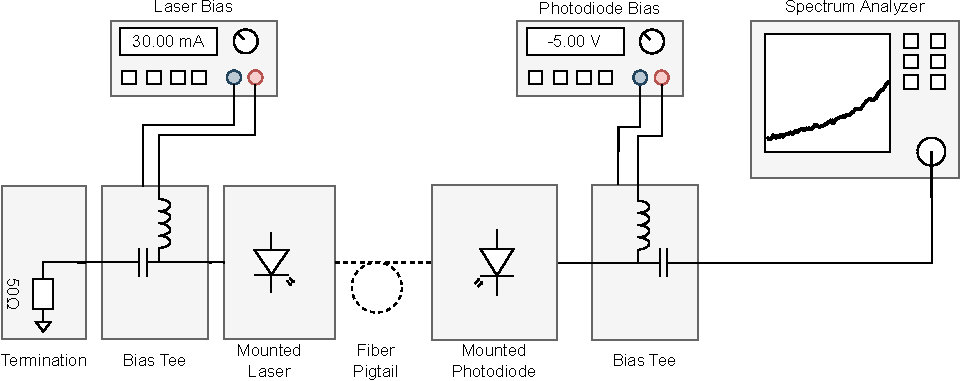
\includegraphics[width=\textwidth]{figures/rin_test.pdf}
    \caption{Diagram of RIN test setup}
    \label{fig:rin_test_setup}
\end{figure}

To compute the link noise alone, we subtract the ``dark'' noise from the measurement with the laser on.
Then, we compute the noise power into the spectrum analyzer from the photodiode's DC shot noise, and subtract that as well to result in just the laser's noise power.
Finally, as the noise power is proportional to $\overline{p_L^2}$, we divide by DC photocurrent's equivalent power to compute RIN, given by
\begin{equation}
    \text{RIN}~(\text{dB/Hz}) = 10\log10{\frac{S_T - S_{RX}-2qI_{PD}Z_0}{I_{PD}^2Z_0}} \,,
\end{equation}
where $S_T$ is the total power spectral density, $S_{RX}$ is the measured ``dark'' power spectral density, $I_{PD}$ is the DC photocurrent, $q$ is the electron charge, and $Z_0$ is the input impedance of the spectrum analyzer.
We then repeat this measurement as a function of bias.
The result of this experiment is shown in \autoref{fig:rin}.
The ripple in this measurement is due to the mismatch between the high impedance photodiode and the length of transmission line and bias tee before the \qty{50}{\ohm} spectrum analyzer input.
Missing data are due to the sensitivity limitations of the spectrum analyzer.

\begin{figure}[ht!]
    \centering
    \includestandalone[mode=buildnew]{figures/rin}
    \caption[Measured RIN of an AGx laser]{Measured RIN of an AGx laser. Top to bottom: \qty{10}{\mA} to \qty{50}{\mA} in steps of \qty{4}{\mA}}
    \label{fig:rin}
\end{figure}

To validate our assumptions about RIN, we look at the bias (optical power) response at several frequencies.
To observe the dependence on laser power instead of laser bias current, however, we need to transform the laser current to power via the laser's threshold current $I_{th}$ and slope efficiency $s$.
As we also have measurements of the DC photocurrent, and know the photodiode's responsivity $\eta$ and an approximate less-than-unity gain (loss) of the connector interface $G_O$, we can estimate the optical power from that direction as well.
From the datasheet, $I_{th}$\qty{=8}{\mA}, $s$\qty{=0.315}{\W/\A}, $\eta$\qty{=0.93}{\A/\W}.
We estimate $G_O$ to be \num{0.98}.

\begin{figure}[ht!]
    \centering
    \includestandalone[mode=buildnew]{figures/laser_pi}
    \caption{Laser output power vs. laser current and DC photocurrent}
    \label{fig:laser_pi}
\end{figure}

Looking at the response in \autoref{fig:laser_pi}, we observe that the datasheet values and our assumptions agree.
This implies we can use either conversion factor to compute laser power instead of disconnecting the laser and attaching it to an optical power meter.

\begin{figure}[ht!]
    \centering
    \includestandalone[mode=buildnew]{figures/rin_v_power}
    \caption{Measured RIN of an AGx laser vs laser output at three frequencies}
    \label{fig:rin_v_power}
\end{figure}

\autoref{fig:rin_v_power} shows the RIN versus laser power at a few frequencies.
We observe the steep increase in RIN at low laser power due to spontaneous emission, and the linear section due to shot noise at higher power, matching our prediction.

To aid in analysis, we ignore the frequency dependence for now and fit a simple quadratic model at \qty{1.5}{\GHz}
\begin{equation}
    \text{RIN}_\text{Model} = -131.2 - 5.5P + 0.19P^2 \,,
    \label{eq:rin_model}
\end{equation}
where $P$ is the laser output power in mW, also plotted in \autoref{fig:rin_v_power}.

Now that we understand the bias and frequency response of RIN, we continue with our noise analysis.
In the small signal case, the laser appears as a small resistor $R_L$, with deviations in current manifesting as deviations in the intensity of the light following the slope efficiency of the laser.
The RIN is then superimposed over this modulated light, creating a mean square deviation over the DC optical power $P$ following
\begin{equation}
    \overline{p_L^2} = \text{RIN}\cdot P^2B \,.
\end{equation}
Finally, the light is attenuated by the less-than-unity gain of the fiber, $G_O$, and is converted back into current following the photodiode's responsivity.
As the laser is biased to a fixed optical output from which it is then modulated, the DC photocurrent generates shot noise in the photodiode following
\begin{equation}
    \overline{i_P^2} = 2qI_PB = 2qPG_O\eta B \,.
\end{equation}
The equivalent noise circuit for this system is shown in \autoref{fig:rfof_noise}.

We simplify this circuit by combining the dependent sources and moving the noise currents forward towards the output, Port 2.
The total current gain between the laser input and the photodiode is
\begin{equation}
    g_i = sG_O\eta \,.
\end{equation}
Noise in the optical power of the laser manifests as noise in the photocurrent, scaled by the square of the passive gain of the fiber and the photodiode responsivity, $(G_O\eta)^2$.
As the shot noise and RIN are uncorrelated, the total noise current is their sum given by
\begin{equation}
    \overline{i_\text{Out}^2} = \overline{p_L^2}(G_O\eta)^2 + \overline{i_P^2} = PG_O\eta B(PG_O\eta\cdot\text{RIN} + 2q) \,.
\end{equation}
The simplified, output-referred circuit is shown in \autoref{fig:rfof_noise_output}.
\begin{figure}[ht!]
    \centering
    \includestandalone[mode=buildnew]{figures/rfof_output_current}
    \caption{RFoF output-referred current noise}
    \label{fig:rfof_noise_output}
\end{figure}

It is usual to work in input-referred noise and here we encounter the first quirk in noise analysis, where instead of simply referring $\overline{i_\text{Out}^2}$ to the input by $g_i^2$, we must consider the impact of the source termination.
Definitionally, noise figure is the degradation in SNR, where the ``signal'' originates from a power source, i.e., with a source impedance.
This is emblematic of the difficulty in this type of analysis, as it would seem that moving the currents forward in the previous case is the same as moving them backwards towards the input.
However, the subtle distinction here is that moving forward is asking, "how does current changing at the input branch manifest as current at the output", which depends solely on the gain, whereas moving backwards is asking, "what equivalent current at the input would manifest as current at the output", which depends on the circuitry attached to the input.
We begin to solve this problem by working backwards, starting with the current we want at the input under the source termination condition and working towards the output.

\begin{figure}[ht!]
    \centering
    \includestandalone[mode=buildnew]{figures/rfof_input_current}
    \caption{RFoF input-referred current noise}
    \label{fig:rfof_noise_input}
\end{figure}

In this configuration, we use the current divider to find
\begin{equation}
    i_L = i_\text{In}\frac{R_S}{R_L+R_S} \,.
\end{equation}
Then, we use the current gain to move to the output
\begin{equation}
    i_\text{Out} = g_ii_\text{In}\frac{R_S}{R_L+R_S} \,.
\end{equation}
Finally, we solve for $i_\text{In}$ in terms of $i_\text{Out}$, and take the time average of the square
\begin{equation}
    \overline{i_\text{In}^2} = \frac{\overline{i_\text{Out}^2}}{g_i^2}\left(\frac{R_L}{R_S}+1\right)^2 \,.
\end{equation}

To find the noise figure, we use the relation
\begin{equation}
    F = \frac{\overline{i_\text{Total}^2}}{\overline{i_S^2}} = \frac{\overline{i_\text{In}^2} + \overline{i_S^2}}{\overline{i_S^2}} = \frac{\overline{i_\text{In}^2}}{\overline{i_S^2}} + 1 \,,
\end{equation}
where $\overline{i_S^2}$ is the thermal noise in the generator, defined as
\begin{equation}
    \overline{i_S^2} = 4k_BT_0G_SB \,,
\end{equation}
where $G_S$ is the source conductance and $T_0$ \qty{=290}{\K} (IEEE standard).
Combining these equations yield
\begin{equation}
    F = 1 + \frac{\overline{i_\text{Out}^2}\left(\frac{R_L}{R_S}+1\right)^2}{4k_BT_0G_SBg_i^2} \,.
\end{equation}
Finally, as we prefer to work in equivalent noise temperature, we use $T_e = T_0(F-1)$, we find
\begin{equation}
    T_e  = \frac{PR_S}{4k_Bs^2G_O\eta}\left(PG_O\eta\cdot\text{RIN} + 2q\right)\left(\frac{R_L}{R_S}+1\right)^2 \,.
    \label{eq:link_noise}
\end{equation}

This equivalent noise temperature result gives insight into the behavior of the link under different source impedances.
If we are free to choose $R_S$ through matching, we would want to know what $R_S$ provides the best noise performance.
We solve for this quantity by minimizing \autoref{eq:link_noise}, finding the $R_S$ that solves $\delta T_e/\delta R_s=0$.
Taking the positive solution of the quadratic yields
\begin{equation}
    R_{S,\text{Opt}} = R_L \,.
\end{equation}
This follows from the fact that all the noise sources are not electrically influenced by the source impedance, so by conjugate matching the laser, we maximize the link's gain and therefore minimize the input-referred noise.
In this case, we can find the minimum noise temperature of
\begin{equation}
    T_\text{Min}  = \frac{PR_L}{k_Bs^2G_O\eta}\left(PG_O\eta\cdot\text{RIN} + 2q\right) \,,
    \label{eq:min_link_noise}
\end{equation}
which is a ratio of
\begin{equation}
    \frac{T_e}{T_\text{Min}} = \frac{(R_S+R_L)^2}{4R_SR_L} \,,
\end{equation}
or \num{3.025} for $R_S$ \qty{=50}{\ohm} and $R_L$ \qty{=5}{\ohm}
The plot for minimum noise alongside the \qty{50}{\ohm} noise is shown in \autoref{fig:link_noise}.
This figure uses typical parameters for our laser\footnote{\url{https://www.agxtech.com/PDF/PLMR3+Rev+4.0.pdf}}, which has a RIN following our model in \autoref{eq:rin_model}, a slope efficiency $s$ of \qty{0.315}{\watt/\ampere}, and a slope impedance of \qty{5}{\ohm} and for our photodiode\footnote{\url{https://www.agxtech.com/PDF/PPDA+R5.6.pdf}}, which has a slope efficiency $\eta$ of \qty{0.93}{\ampere/\watt}.
The conclusion from this plot is that for laser powers between \qty{8}{\mW} and \qty{12}{\mW}, the noise is about the same, within a factor of 2, and remains that way as we increase the loss.

\begin{figure}[ht!]
    \centering
    \includestandalone[mode=buildnew]{figures/link_noise}
    \caption[RFoF link noise]{RFoF link noise ($R_S=$ \qty{50}{\ohm} (solid) and optimal (dotted)) versus optical attenuation}
    \label{fig:link_noise}
\end{figure}

With $T_e(R_S)$ and $R_{S,\text{Opt}}$, we have essentially derived the noise parameters of the RFoF link.
Notably missing from this analysis are the parasitics of the components, the series inductance of the leads of the packaged coaxial laser and photodiode, and the junction capacitance of the photodiode.
To minimize noise, as we have seen, we will want to power match at the input of the network.
As such, any inductance at the input will need to be tuned out in addition to matching the slope resistance.

\subsubsection{S Parameters}

In analyzing the gain and reflection coefficients of the RFoF link, it is more convenient to analyze S parameters instead of voltages and currents.
However, determining the S parameters directly from the \autoref{fig:rfof_noise} model is nontrivial due to the dependent sources.
Instead, it would be easier to consider the Y parameters and convert using the well-known formula.
The Y parameters of \autoref{fig:rfof_noise} are
\begin{equation}
    Y_\text{Link} = \frac{1}{R_L}\begin{bmatrix}
        1 & 0 \\ s\eta G_\text{O} & 0
    \end{bmatrix} \,.
\end{equation}
Converting to S parameters gives
\begin{equation}
    S_\text{Link} = \begin{bmatrix}
        \dfrac{R_L-Z_0}{R_L+Z_0} & 0 \\\\[0.2em] \dfrac{2Z_0s\eta G_\text{O}}{R_L+Z_0} & 1
    \end{bmatrix} \,.
    \label{eq:unmatched_rfof_s}
\end{equation}

$S_{11}$ of this result is as expected, it is simply the reflection coefficient of the laser's slope impedance.
$S_{21}$, however, is more nuanced.
If we substitute numbers into this equation such as $Z_0$=\qty{50}{\ohm}, $R_L$=\qty{5}{\ohm} and $s\eta G_\text{Opt}$=\num{0.2}, we find $|S_{21}|^2$=\qty{-8.79}{dB}.
If we ``match'' the laser by setting the characteristic impedance equal to the laser's impedance $R_L=Z_0$, the equation reduces to $s\eta G_\text{Opt}$.
However, using the same device parameters, we find $|0.2|^2$=\qty{-13.98}{\dB}, unintuitively lower gain than before.
The apparent drop in gain is because the equation for $S_{21}$ assumes both the output and input ports have equivalent characteristic impedance, and changing the output impedance changes the power delivered from the photodiode.
It would be more correct to analyze this circuit with an explicit matching network at the input.

For a real load as we are exploring, we can use an ideal transformer at the input as our matching network, which has an ABCD matrix of
\begin{equation}
    A_{TF} = \begin{bmatrix}
        N & 0\\0 & 1/N
    \end{bmatrix} \,.
\end{equation}
We convert the Y matrix of the link to ABCD parameters using the standard equation to arrive at
\begin{equation}
    A_\text{Link} = -\frac{1}{s\eta G_\text{O}}\begin{bmatrix}
        0 & R_L \\ 0 & 1
    \end{bmatrix} \,.
\end{equation}
We  then cascade to get
\begin{equation}
    A_\text{Combined} = -\frac{1}{s\eta G_\text{O}}\begin{bmatrix}
        0 & NR_L \\ 0 & 1/N
    \end{bmatrix} \,.
\end{equation}
And then finally converting to S parameters, we find
\begin{equation}
    S_\text{Combined} = -\frac{1}{Z_0+N^2R_L} \begin{bmatrix}
        Z_0-N^2R_L & 0 \\ 2NZ_0s\eta G_\text{O} & 1
    \end{bmatrix} \,.
\end{equation}
If $N=\sqrt{Z_0/R_L}$, matching to the laser resistance, this reduces to
\begin{equation}
    S_\text{Matched} = \begin{bmatrix}
        0 & 0 \\ -\sqrt{Z_0}s\eta G_\text{O}/\sqrt{R_L} & 1
    \end{bmatrix} \,.
    \label{eq:matched_rfof_s_params}
\end{equation}
Using the same parameters as before, the matched link now has an $|S_{21}|^2$ of \qty{-3.98}{\dB}, or \qty{4.81}{\dB} higher gain than unmatched.
A notable result from this is that positive power gain can be achieved, even though the intrinsic link exhibits a current gain of less than unity.
For example, if $s\eta G_O$\num{=0.2}, $Z_0$\qty{=50}{\ohm}, and $R_L$\qty{=2}{\ohm}, the link's gain $|S_{21}|$ would be unity.
While unintuitive, the transformer acts as a current gain device, for which a given turns ratio will counteract the current loss in the link.
From both the noise and gain perspective, we want to power match the input of the laser.

\subsection{Linearity}

The final metric we evaluate for the RFoF link is the linearity.
If radio frequency interference (RFI) is strong enough, nonlinearity in the signal chain would result in frequency products in addition to the center frequency of the RFI itself.
The strength of these $n$th-order products depends on the strength of the incoming signal and the $n$th derivative of the transfer function of the system.
One way to reduce the impact of this distortion is to simply limit the incoming signal strength.
Doing so, however, is at odds with added noise, as we want to \textit{increase} power before a noisy component to reduce that component's noise impact on the SNR.
To compare RFoF links (bias settings, laser or photodiode choice, etc.), we use ``spurious free dynamic range'' or (SFDR) as a noise-normalized linearity metric.
SFDR is defined as the maximum signal power at the output for which the power of the $n$-th order intermodulation product is equal to the noise power.
This is defined following~\cite{pozarMicrowaveEngineering2012} as
\begin{equation}
    \text{SFDR}_n~(\text{dB})= \frac{n-1}{n}(\text{OIP}n - N_O) \,,
    \label{eq:sfdr}
\end{equation}
where $\text{OIP}_n$ is the $n$th order output intermodulation intercept point and $N_O$ is the output noise power, both defined in dBm.
We only need to consider $n=3$ for narrowband systems, but our radio telescope is more than an octave, so we must consider second order distortion as well, as distortion products from the lower half of the band will appear in the upper half.

\subsection{Experimental Results}

\subsubsection{Noise}

\begin{figure}[ht!]
    \centering
    \includestandalone[mode=buildnew]{figures/link_noise_in}
    \caption[RFoF link input noise temperature]{RFoF link input noise temperature from \qty{10}{\mA} to \qty{50}{\mA} (top to bottom) in steps of \qty{4}{\mA}}
    \label{fig:link_noise_in}
\end{figure}

To validate our noise derivation, we directly measured the link output noise and referred this to the input.
The setup is identical to that used in the RIN characterization, shown in \autoref{fig:rin_test_setup}.
We used a spectrum analyzer as a power meter to measure the noise power, with the link input terminated with a room-temperature load.
In addition to this ``hot'' measurement, we also measured the noise of the receiver, including the ``dark current'' of the photodiode.
Finally, we subtracted the linear noise powers to leave us with just the noise of the link.
Using measured power gain from a network analyzer, we referred the noise power back to the input.

% For this experiment, we used an AGx \textit{PLMR3-A-1-5-S} laser\urlfootnote{http://www.agxtech.com/PDF/PLMR3+Rev+4.0.pdf}.
% We first measured the slope resistance (or equivalent input impedance) by measuring $S_{11}$ on a network analyzer.
% As the laser was mounted to an SMA connected, we measured an open circuit on a connector of the same length to de-embed the effect of the added electrical length.
% After performing the de-embedding, we find the laser's impedance to be \complexqty{5+25j}{\ohm} at \qty{1.5}{\GHz} and \qty{3.1}{\ohm} near DC.

We measured the noise power spectral density on a spectrum analyzer at the output of the photodiode, subtracting the receiver noise.
The input-referred noise temperature in \autoref{fig:link_noise_in} matches our expected result from \autoref{fig:link_noise}, with high laser currents resulting in an input noise temperature of about \qty{60000}{\K} in the band of interest.
While this is an excellent result, we need to consider both the noise and linearity to compute the SFDR.

\subsubsection{Linearity}

\begin{figure}[ht!]
    \centering
    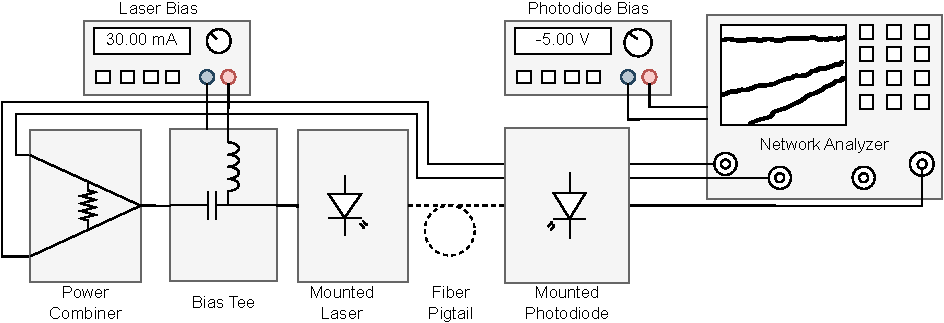
\includegraphics[width=\textwidth]{figures/lin_test.pdf}
    \caption{Diagram of linearity test setup}
    \label{fig:lin_test_setup}
\end{figure}
%
While it is simple to measure noise and gain to validate analytic expressions, linearity is more difficult as we do not have an expression for the actual transfer function of the laser and photodiode pair.
The solution is to probe the individual derivatives of the transfer function by injecting a pair of tones and observing their intermodulation products, derived for reference in \autoref{ch:eqns}.
For the experiment, we inject two closely spaced tones, $\omega_L$ and $\omega_H$ (\qty{1}{\MHz} apart) and observe five tones on the output.
We observe the powers of the two fundamental tones to track the gain, $P_L$ and $P_H$, $\omega_L+\omega_H$ for $\text{IM}_2$ to compute $\text{OIP2}$ via
\begin{equation}
    \text{OIP2}~(\text{dBm}) = P_L+P_H-\text{IM2} \,,
\end{equation}
and $2\omega_H-\omega_L$ for $\text{IM}_{3H}$, and $2\omega_L-\omega_H$ for $\text{IM}_{3L}$ to compute $\text{OIP3}$ via
\begin{align}
    \text{OIP3}~(\text{dBm}) &= \frac{2P_L+P_H-\text{IM3}_{L}}{2}\\
    &= \frac{P_L + 2P_H - \text{IM3}_{H}}{2} \,.
\end{align}
As OIP3 has two unique solutions, we are typically interested in the worst case, which will be the minimum of the two OIP3 results.
For most components, the two terms will be close to equal.
Performing this experiment for the AGx laser and photodiode pair from before, we measured the results shown in \autoref{fig:rfof_oipn}.

\begin{figure}[ht!]%
    \centering
    \subfloat{\includestandalone[mode=buildnew]{figures/laser_oip2}}%
    \quad%
    \subfloat{\includestandalone[mode=buildnew]{figures/laser_oip3}}%
    \caption[RFoF measured OIPn]{RFoF measured OIPn. Red trace is the receiver linearity, black traces bottom to top are laser currents from \qty{10}{\mA} to \qty{50}{\mA} in steps of \qty{2}{\mA}}%
    \label{fig:rfof_oipn}%
\end{figure}

This measurement was performed on a PNA-X network analyzer, utilizing the two independent sources as the two tones incident on the link under test, shown in \autoref{fig:lin_test_setup}.
We used a power combiner to join these two outputs, and calibrated out the loss of the combiner and bias tee to result in an incident power of \qty{-20}{\dBm} for each tone.
The analyzer was then configured to detune the receiver to follow the five tones of interest described earlier, measuring the power directly in dBm.
This measurement includes a correction for the loss in the cable and internals following the photodiode.

Both the IP2 and IP3 results are excellent for this laser, being limited by the dynamic range of the PNA-X in the IP3 measurement.
In the presented range, the gain only changes slightly, from an average of \qty{-5}{\dB} to \qty{-4}{\dB} across the band, with associated input values changing accordingly.
The linearity improves through increased laser power, but then worsens as the device starts to saturate, near \qty{50}{\mA}.

Combining the noise and linearity measurements, we compute the spurious-free dynamic range as defined in \autoref{eq:sfdr}, shown in \autoref{fig:rfof_sfdr}.
%
\begin{figure}[ht!]%
    \centering
    \subfloat{\includestandalone[mode=buildnew]{figures/rfof_sfdr2}}%
    \quad%
    \subfloat{\includestandalone[mode=buildnew]{figures/rfof_sfdr3}}%
    \caption[Spurious-free dynamic range for the intrinsic RFoF link]{Spurious-free dynamic range for the intrinsic RFoF link. Traces bottom to top are laser currents from \qty{10}{\mA} to \qty{50}{\mA} in steps of \qty{2}{\mA}. Noise power is the measured intrinsic link noise under \qty{100}{\kHz} of noise equivalent bandwidth.}%
    \label{fig:rfof_sfdr}%
\end{figure}
%
Here, we see that we are limited primarily by the 2nd-order linearity, although it is important to note that after \qty{1}{\GHz}, the power in the second order tone (\qty{2}{\GHz}) is out of band and will be filtered out).
At high laser powers, in the band of \SIrange{0.7}{2}{\GHz}, we can expect SFDR of better than \qty{60}{\dB} for the intrinsic RFoF link.

As the SFDR falls off at high laser power while the noise improves, we find the optimum laser bias of around \qty{38}{\mA} shown in \autoref{fig:sfdr2_sweep}.

\begin{figure}[ht!]
    \centering
    \includestandalone[mode=buildnew]{figures/sfdr2_sweep}
    \caption{Spurious-free dynamic range for the RFoF link vs laser current}
    \label{fig:sfdr2_sweep}
\end{figure}

\subsection{Long-Haul RFoF}

\begin{figure}[ht!]
    \centering
    \includestandalone[mode=buildnew]{figures/scattering_linearity}
    \caption[Linearity metrics for single- and double- isolated lasers]{Linearity metrics for single- and double- isolated lasers at 0 and \qty{20}{\km}. Both lasers are operated at \qty{40}{mA}.}
    \label{fig:scattering_linearity}
\end{figure}

The final piece of the RFoF puzzle involves the consequences of the exceptionally long fiber that connects the most remote antennas in the telescope to the digitizers.
Current estimates predict the longest fiber lengths will be about \qty{20}{\km}.
As the lasers operate at $1310\,\text{nm}$, the effective loss in standard single-mode fiber is around \qty{0.5}{\dB/\km}.
\autoref{fig:link_noise} indicates that the resulting \qty{10}{\dB} of optical loss (\qty{20}{\dB} in RF power loss) will result in about a factor of four increase in noise.
This is still an acceptable noise level, as there can be a significant amount of gain before the link.

In initial experiments with a \qty{20}{\km} spool on the bench, linearity and noise both worsened significantly more than what was expected.
We believe the origin of these effects are reflections off imperfect connectors and Rayleigh backscattering, coupled with poor isolation in the laser and laser chirp.
While simple reflections are a well-known issue in RFoF links, the induced distortion due to the increased effect of Rayleigh backscattering in long fibers combined with the laser chirp is more nuanced.
Only recently has this effect been discussed in the context of radio astronomy~\cite{periniRadioFrequencyFiber2022,nanniControllingRayleighBackscatteringInducedDistortion2020}.

Rayleigh backscattering is a phenomenon in optical fiber where imperfections in the refractive index results in scattering.
While this would typically manifest as a linear effect (and is the dominant component of loss in fiber optic links~\cite{kanamoriTransmissionLossOptical2021}), the interaction with the chirp of the laser results in nonlinear effects.
Chirp is the change in instantaneous optical frequency of the laser as it is directly modulated.
As Rayleigh backscattering sends a reflected wave back into the laser, the time-dependence of chirp results in the different optical frequencies mixing and retransmitting, resulting in a distorted signal.

There are a few ways one could mitigate the distortion introduced from chirp and scattering.
The most straightforward approach would be to use a lower chirp laser, or to use an external modulator where there would be no chirp.
Both of these solutions, however, are typically expensive.
The solution for one radio telescope (the SKA)~\cite{nanniControllingRayleighBackscatteringInducedDistortion2020} is to introduce a dithering tone.
This low frequency modulation added on top of the RF modulation results in decoherence of the scattered light and the light emitted from the gain cavity of the laser.
This solution, however, requires additional hardware and filtering.
The most simple solution is to instead purchase lasers with more optical isolation built in, or add in-line isolators in the path of the fiber near the laser.
For most vendors, a double isolator (which increases the optical isolation by \qty{20}{\dB}) is on the order of a \$10 increase in cost.

We find that adding additional isolators is an effective way to reduce the nonlinearities introduced by Rayleigh backscattering by repeating the earlier tests on the bench with a \qty{20}{\km} spool\footnote{Thank you, Courtney!}, shown in \autoref{fig:scattering_linearity}.
In this figure, the top row are tests with \qty{0}{\km} of fiber, with the laser and photodiode directly connected.
The bottom row adds a \qty{20}{\km} spool of single-mode fiber between the two.
The left column shows OIP2 and the right column shows OIP3.
All four measurements are shown for the single- and double-isolated lasers.

\begin{figure}[ht!]
    \centering
    \includestandalone[mode=buildnew]{figures/scattering_noise}
    \caption[Noise temperature for single- and double- isolated lasers]{Noise temperature for single- and double- isolated lasers at \qty{0}{\km} (dotted) and \qty{20}{\km} (solid). Both lasers are operated at \qty{40}{mA}}
    \label{fig:scattering_noise}
\end{figure}

From \autoref{fig:scattering_linearity}, it is clear that at \qty{20}{\km} we observe Rayleigh scattering as the linearity for the single-isolated laser is significantly lower.
Adding the double isolator improves the linearity for both second and third order distortion.
It is important to note, however, that the overall output intercept points have dropped in the case of the long fiber.
This is due to the fiber introducing \qty{10}{\dB} of loss, and the primary distortion mechanism is from the laser itself.
If you add the \qty{10}{\dB} of loss back to the \qty{20}{\km} numbers, the double-isolated intercept points match the \qty{0}{\km} measurements, matching our expectations.

We can see similar behavior in noise by measuring the devices in the same manner as described earlier.
The results are shown in \autoref{fig:scattering_noise}\footnote{Ripples are due to uncalibrated cables that connect to the bare diodes, as this measurement was performed on a spectrum analyzer with a tracking generator and not a network analyzer}.
With the single-isolator laser, the noise increases by more than an order of magnitude when we add the \qty{20}{\km} of fiber, which is much more than the predicted results from \autoref{fig:link_noise}.
With the double-isolated laser, however, the noise is almost exactly what we predict of around \qty{2e5}{\K}.

Adding a double isolator is a simple, low-cost solution that significantly improves the performance of the link in the long-haul limit.
Additionally, doing so does not reduce performance in the short-fiber distances.
The output power of the laser is lower in the double-isolated case due to the doubled insertion loss of the isolator, but this only mildly increases the noise.

\section{System Design}

\subsection{Link Budget}

For the DSA-2000, we are presented with a few key science requirements that induce engineering requirements.
For us, the most important metric is survey speed.
Our ability to survey the sky to high sensitivity with a fast cadence is one reason this instrument will be impactful.
Survey speed is a consequence of the radiometer equation, where we compute the RMS uncertainty in a noise measurement by 
\begin{equation}
    \sigma_T = \frac{T_\text{Sys}}{\sqrt{B\tau}} \,,
\end{equation}
given system temperature $T_\text{Sys}$, bandwidth $B$ and integration time $\tau$.
If our goal is to have high confidence in our results, say $5\sigma$ and the telescope has some fixed bandwidth, we have two ``free'' parameters: $T_\text{Sys}$ and $\tau$.
These are free in the sense that $T_\text{Sys}$ is an engineering requirement and $\tau$ is an operational requirement.
If $T_\text{Sys}$ were very low, we could integrate over much less time to achieve the same statistical result.
For a large survey, we must perform this integration for every piece of the sky we want to observe.
As such, driving down $T_\text{Sys}$ is critical for the survey speed performance, quadratically so.

To not significantly perturb the survey speed, we chose to place a limit of no more than \qty{1}{\K} added to $T_\text{Sys}$ from electronics following the LNA.
As the LNA has \qty{\approx35}{\dB} of gain, this implies a maximum tolerable noise of \qty[group-digits = false]{\approx3100}{\K} at the output of the LNA.

Next, we focus on the total gain requirement.
The amount of absolute power required to drive the digitizers is dependent on the exact digitizer we use.
The current design uses the 12-bit AD9207\footnote{\raggedright\url{https://www.analog.com/media/en/technical-documentation/data-sheets/ad9207.pdf}} from Analog Devices.
The full-scale peak-to-peak input voltage is \qty{1.475}{\V} across the differential \qty{100}{\ohm} input.
We want to set the gain of the analog signal path such that the astronomical signal exercises about three bits~\cite{bianchi2008adc}.
A detectable signal must be above the device's quantization noise, reducing the effective bit-depth of the ADC to an ``effective number of bits'' (ENOB).
Our ADC has an ENOB of about 9 at \qty{2}{\GHz}.
This implies that three bits correspond to a peak-to-peak voltage of \qty{23.05}{\mV}, or \qty{-31.78}{\dBm} into the \qty{100}{\ohm} differential input.
At the input of the analog signal path, $T_\text{Sys}$ induces a noise power of \qty{-93.48}{\dBm} (\qty{25}{\K} across our \qty{1.3}{\GHz} bandwidth).
Therefore, we require at least \qty{61.7}{\dB} of gain.
About \qty{35}{\dB} of gain is covered by the LNA, leaving only \qty{26.7}{\dB} needed for the remainder of the ASP.

Finally, we must consider linearity.
The signal levels from astronomical sources will be incredibly faint, so their intermodulation products are unimportant.
Unfortunately, radio frequency interference (RFI) can be terribly strong, wreaking havoc on our science data.
The impact of RFI can be categorized into three domains.
First, if the RFI is faint enough to generate intermodulation products beneath the power of $T_\text{Sys}$, all we must do is flag the carrier channels as contaminated.
Second, the RFI power could be strong enough to generate intermodulation products that also contaminate the science band, implying we would need to flag more than the channel of the RFI.
Finally, the RFI could be so strong that we compress the amplifiers or saturate the ADC, resulting in an unusable signal path.
In the final case, there is not much that can be done in ASP design, depending on what saturates first.
If everything were linear, this gives us \qty{\approx 50}{\dB} of headroom between the ADC noise and the brightest RFI we can tolerate before the ADCs saturate.
This motivates using highly linear amplifiers after the LNA, such that we only need to worry about the ADC.
In the first and second cases, we can derive a constraint in the second and third order intermodulation terms if we want the intermodulation power to be no more than some fraction of the noise power in a channel.

If the signal chain has \qty{61.7}{\dB} of gain and the full-scale power of the ADC is \qty{4.34}{\dBm}, RFI will saturate the ADC at $P_\text{RFI}=$\qty{-57.36}{\dB} into the LNA.
If we constrain the linearity such that the ASP does not generate intermodulation products higher than the noise level of $P_N=$\qty{-93.48}{\dBm} at the input, then we can compute lower limits on the input second-order intercept as $\text{IIP2} = 2P_\text{RFI} - P_N$\qty{=-21.23}{\dBm} and third-order intercept as $\text{IIP3} = (3P_\text{RFI} - P_N)/2$\qty{=-39.29}{\dBm}.
Referred to the output under \qty{61.7}{\dB} of gain, these bounds are an OIP2 and OIP3 of \qty{40.46}{\dBm} and \qty{22.4}{\dBm}, respectively.

\subsection{Cascade Analysis}

To optimize the analog signal path, we compute the input-referred noise and total cascaded linearity.
Computing the total link noise follows from the Friis cascaded noise equation
\begin{equation}
    T_\text{In} = T_\text{LNA} + \frac{T_1}{G_\text{LNA}} + \frac{T_2}{G_\text{LNA}G_2} \dots \,,
\end{equation}
where each subsequent noise contributor is divided by the available gain of all the components before it.
Linearity, however, is again a bit tricky.
As the intermodulation powers are deterministic, they may be in-phase and add coherently.
Following the derivation in~\cite{pozarMicrowaveEngineering2012}, we find the total OIP3 of a cascaded system with coherent products as
\begin{equation}
    \text{OIP3}~(\text{W}) = \left(
    \frac{1}{G_n\text{OIP3}_{{n-1}}} + \frac{1}{\text{OIP3}_{n}}
    \right)^{-1} \,,
\end{equation}
where $G_n$ is the gain of the $n$th component along with its $\text{OIP}_{3_n}$, $\text{OIP}_{3_{n-1}}$ is the cumulative OIP$_3$ through the previous $n-1$ stages.
All of these calculations are performed in linear units.
This equation is a worst-case estimate, assuming every intermodulation product adds coherently.
This will never be the case as there is a relatively random distribution of cable lengths, interconnects, and component phase delays.
As such, we can approximate the phases between each stage to be random, and compute the associated cascaded intercept point as
\begin{equation}
    \text{OIP3}~(\text{W}) = \left(
    \frac{1}{G_n^2\text{OIP3}_{{n-1}}^2} + \frac{1}{\text{OIP3}_{n}^2}
    \right)^{-1/2} \,.
\end{equation}
We can then input-refer these quantities by dividing by the accumulated gain as
\begin{equation}
    \text{IIP}n = \text{OIP}n /G \,.
\end{equation}
Stated another way, if we assume the intermodulation terms have random phase, then their powers would add.
The derivation for 2nd order distortion and cascade analysis can be found in \autoref{ch:eqns}.

Using these results, we compute the cascaded behavior for all the components along the analog signal path, shown in \autoref{tab:casc_asp}.
Our noise only increases by \qty{\approx0.7}{\K}, beneath our requirement of \qty{1}{\K}.
The total gain is \qty{74.7}{\dB}, with adjustable attenuators allowing for control.
We set the attenuators to match our gain requirement and to maximize dynamic range.
Finally, the cascaded OIP2 and OIP3 are \qty{45.83}{\dB} and \qty{33.57}{\dBm} respectively, exceeding our requirements.

\newpage
\begin{landscape}
\begin{table}[!htp]\centering
\caption[Cascade analysis of analog signal path]{Cascade analysis of analog signal path. Included are coherent (Coh.) and random (Rand.) output intercept points. Noise at the input LNA represents the entire system noise temperature. Laser noise is assuming a worst-case of \qty{1e6}{K}. Laser linearity uses the double-isolator result from \autoref{fig:scattering_linearity}. Passive components are taken to have infinite linearity.}\label{tab:casc_asp}
\scriptsize
\begin{tabular}{lr|cccc|ccccccc}\toprule
& &\multicolumn{4}{c}{Component} &\multicolumn{6}{c}{Cascaded} \\\cmidrule{3-12}
Description &Part Number &Gain  &Noise&OIP2 &OIP3 &Acc. Gain &Noise &OIP3 Coh. &OIP3 Rand. &OIP2 Coh. &OIP2 Rand. \\
 & & (dB) & (K) & (dBm) & (dBm) & (dB) & (K) & (dBm) & (dBm) & (dBm) & (dBm) \\\midrule
LNA             & ksWBLNAv2   & 35   & 25     & 22 & 16 & 35   & 25    & 16    & 16    & 22    & 22    \\
Cable           & -           & -3   & 288.63 & -- & -- & 32   & 25.09 & 13    & 13    & 18.99 & 19 \\
Bias Tee        & Lumped      & -0.1 & 6.75   & -- & -- & 31.9 & 25.10 & 12.9  & 12.9  & 18.88 & 18.9 \\
BPF             & Lumped      & -2   & 169.62 & -- & -- & 29.9 & 25.21 & 10.9  & 10.9  & 16.88 & 16.9 \\
Amplifier       & PGA-105     & 15   & 170    & 49 & 39 & 44.9 & 25.38 & 25.69 & 25.89 & 30.75 & 31.82 \\
External Filter & -           & 0    & 0      & -- & -- & 44.9 & 25.38 & 25.69 & 25.89 & 30.72 & 31.82 \\
Attenuator      & F1958       & -2   & 169.62 & 80 & 64 & 42.9 & 25.38 & 23.69 & 23.89 & 28.69 & 29.82 \\
Amplifier       & PGA-105     & 15   & 170    & 49 & 39 & 57.9 & 25.38 & 35.83 & 37.44 & 39.93 & 43.41 \\
Attenuator      & PAT-1220C   & -3   & 288.63 & -- & -- & 54.9 & 25.39 & 32.83 & 34.44 & 36.87 & 40.41 \\
Amplifier       & PGA-105     & 15   & 170    & 49 & 39 & 69.9 & 25.39 & 38.47 & 38.98 & 44.29 & 48.11 \\
BFP             & Lumped      & -1   & 75.09  & -- & -- & 68.9 & 25.39 & 37.47 & 37.98 & 43.17 & 47.1 \\
Attenuator      & PAT-1220C   & -3   & 288.63 & -- & -- & 65.9 & 25.39 & 34.47 & 34.98 & 40.08 & 44.1 \\
Bias Tee        & Lumped      & -0.1 & 6.75   & -- & -- & 65.8 & 25.39 & 34.37 & 34.88 & 39.89 & 44 \\

RFoF Link       & -           & -25  & 1E6    & 20 & 0  & 40.8 & 25.66 & -0.48 & -0.02 & 11.06 & 16.46 \\

Bias Tee        & Lumped      & -0.1 & 6.75   & -- & -- & 40.7 & 25.66 & -0.58 & -0.12 & 10.95 & 16.36 \\
Attenuator      & PAT-1220C   & -3   & 288.63 & -- & -- & 37.7 & 25.68 & -3.58 & -3.12 & 7.95  & 13.36 \\
Amplifier       & PGA-105     & 15   & 170    & 49 & 39 & 52.7 & 25.71 & 11.42 & 11.88 & 22.53 & 28.32 \\
Attenuator      & F1958       & -3   & 288.63 & 80 & 64 & 49.7 & 25.71 & 8.42  & 8.88  & 19.52 & 25.32 \\
BPF             & Lumped      & -1   & 75.09  & -- & -- & 48.7 & 25.71 & 7.42  & 7.88  & 18.51 & 24.32 \\
Amplifier       & PGA-105     & 15   & 170    & 49 & 39 & 63.7 & 25.72 & 22.32 & 22.88 & 32.16 & 38.88 \\
Attenuator      & PAT-1220C   & -3   & 288.63 & -- & -- & 60.7 & 25.72 & 19.32 & 19.88 & 29.14 & 35.88 \\
Amplifier       & PGA-105     & 15   & 170    & 49 & 39 & 75.7 & 25.72 & 33.05 & 34.57 & 40.21 & 46.83 \\
AA Filter       & Distributed & -1  & 75.09   & -- & -- & 74.7 & 25.72 & 32.05 & 33.57 & 39.13 & 45.83 \\
ADC             & AD9207 & & & & & & & & & & \\
\bottomrule
\end{tabular}
\end{table}
\end{landscape}
\newpage

\subsection{FTX and FRX Boards}

\begin{figure}[ht!]%
    \centering
    \subfloat{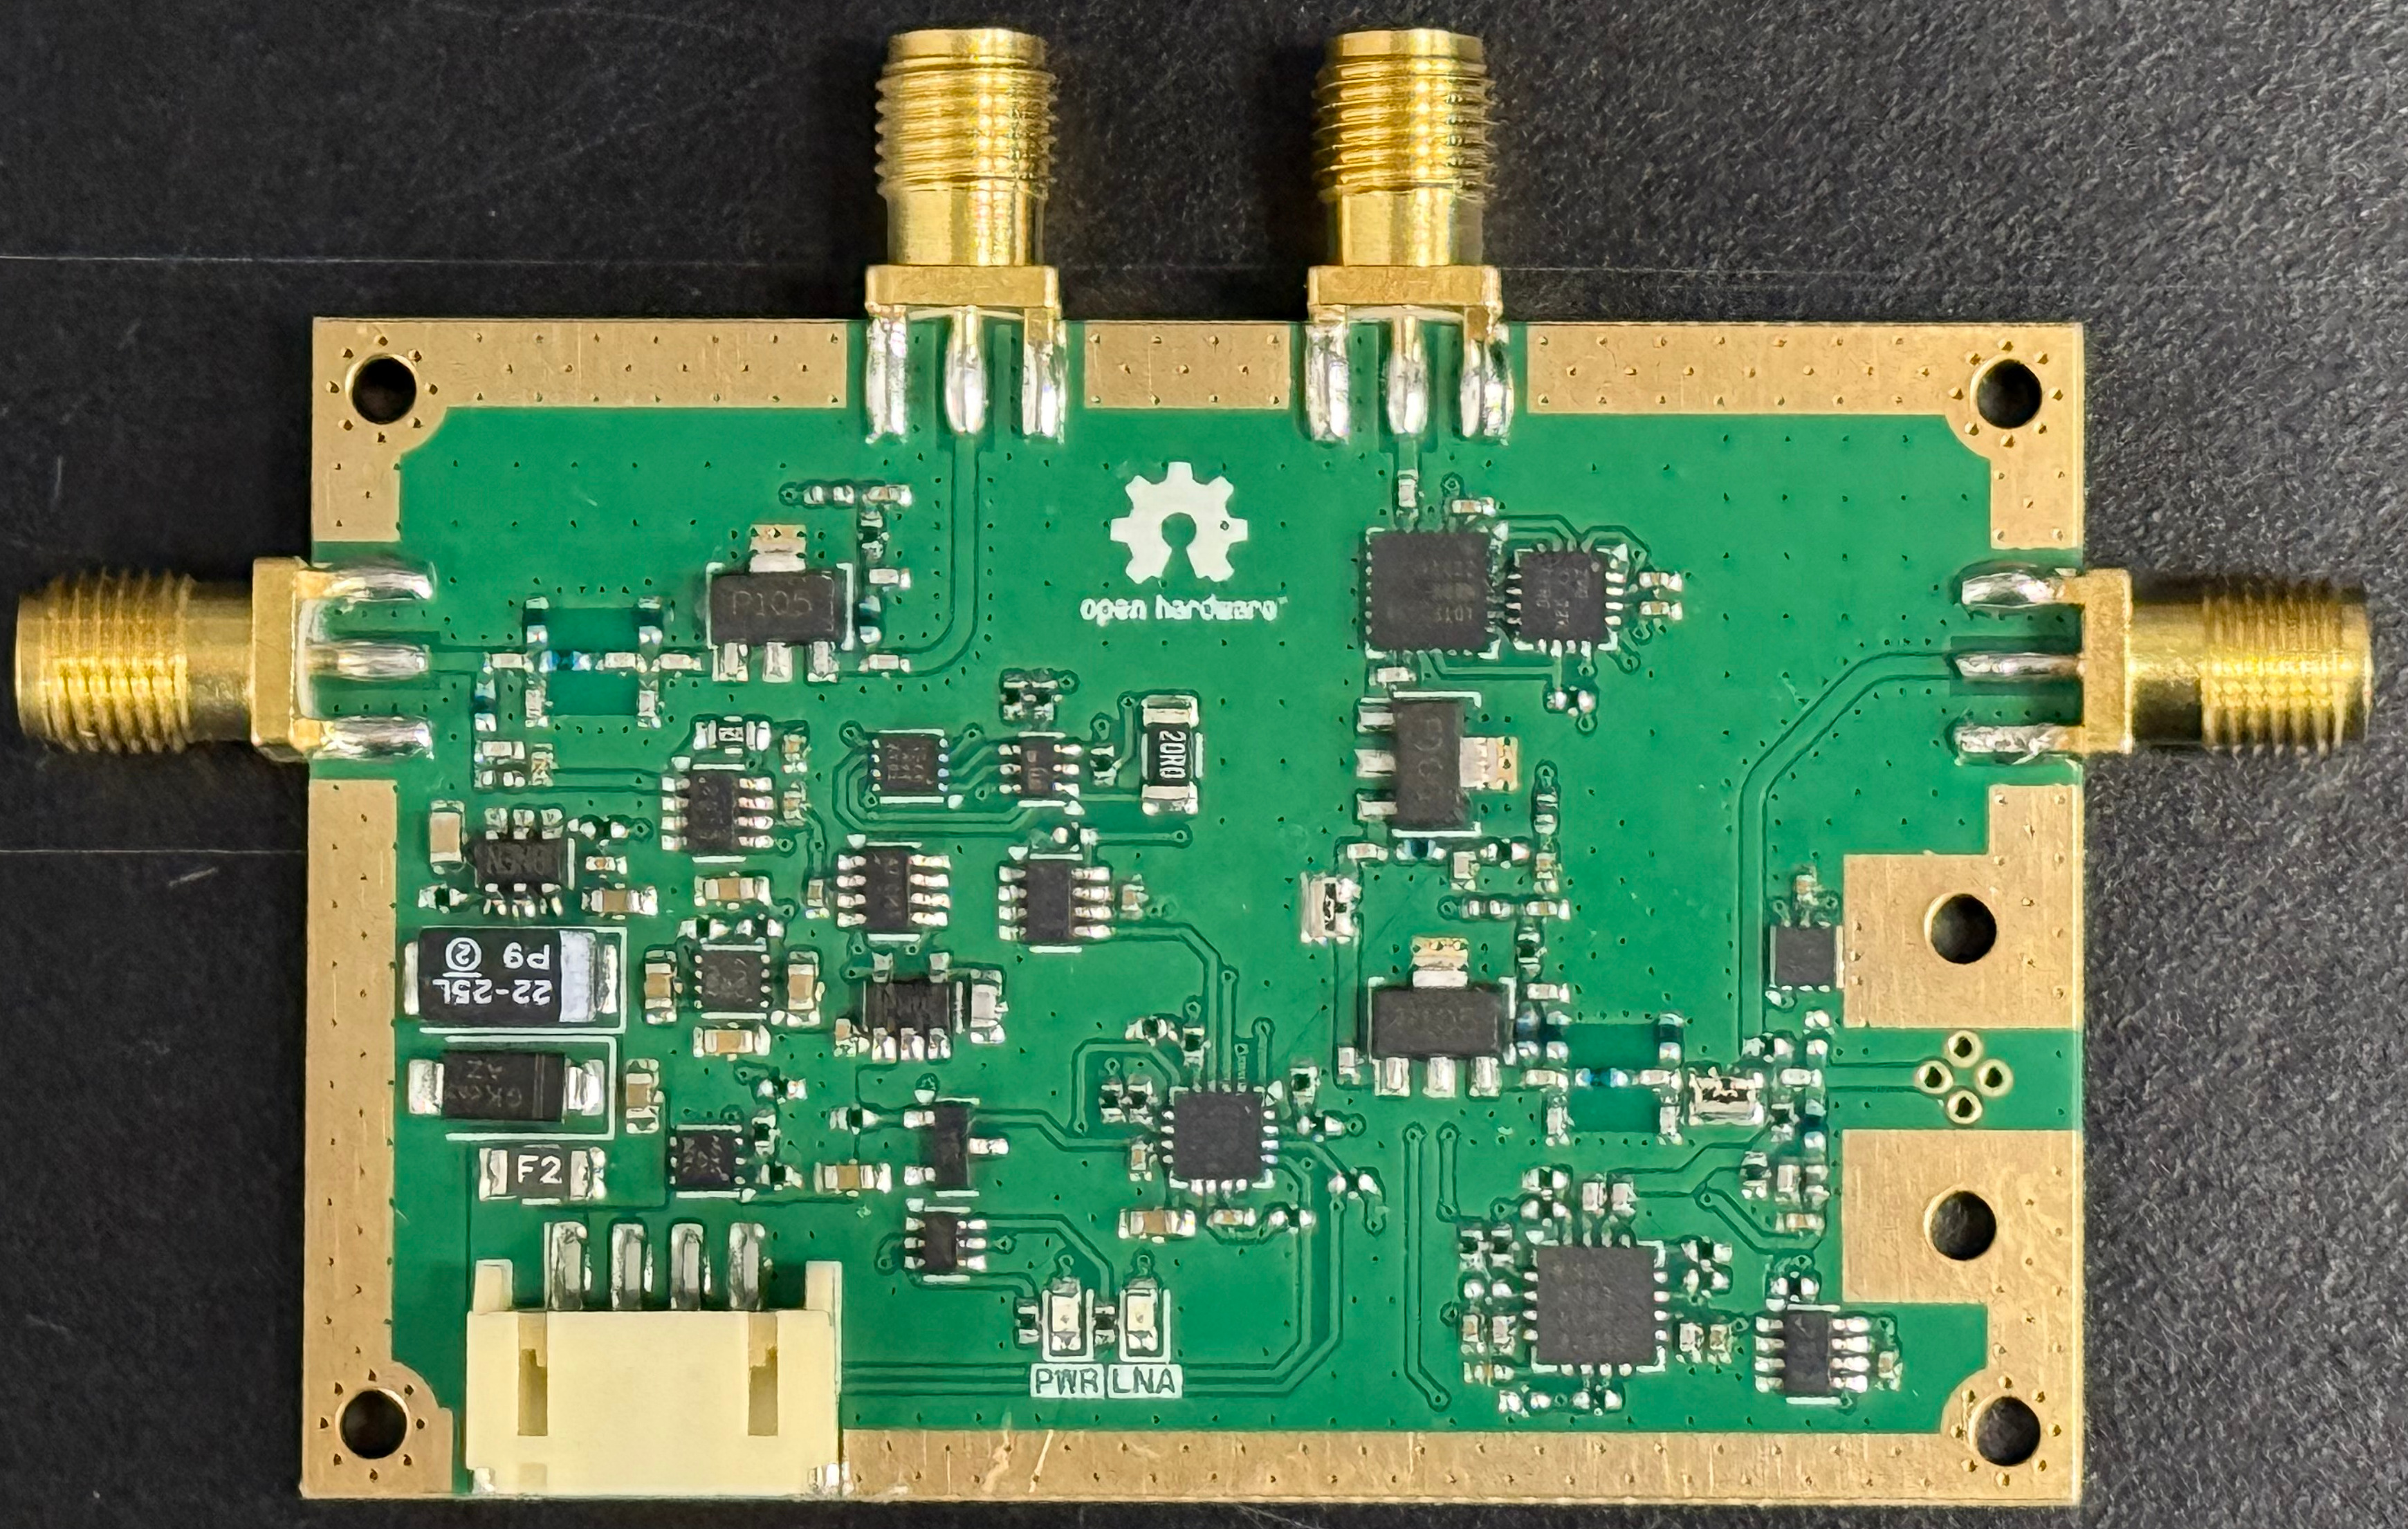
\includegraphics[height=4cm]{figures/ftx.jpg}}%
    \quad%
    \subfloat{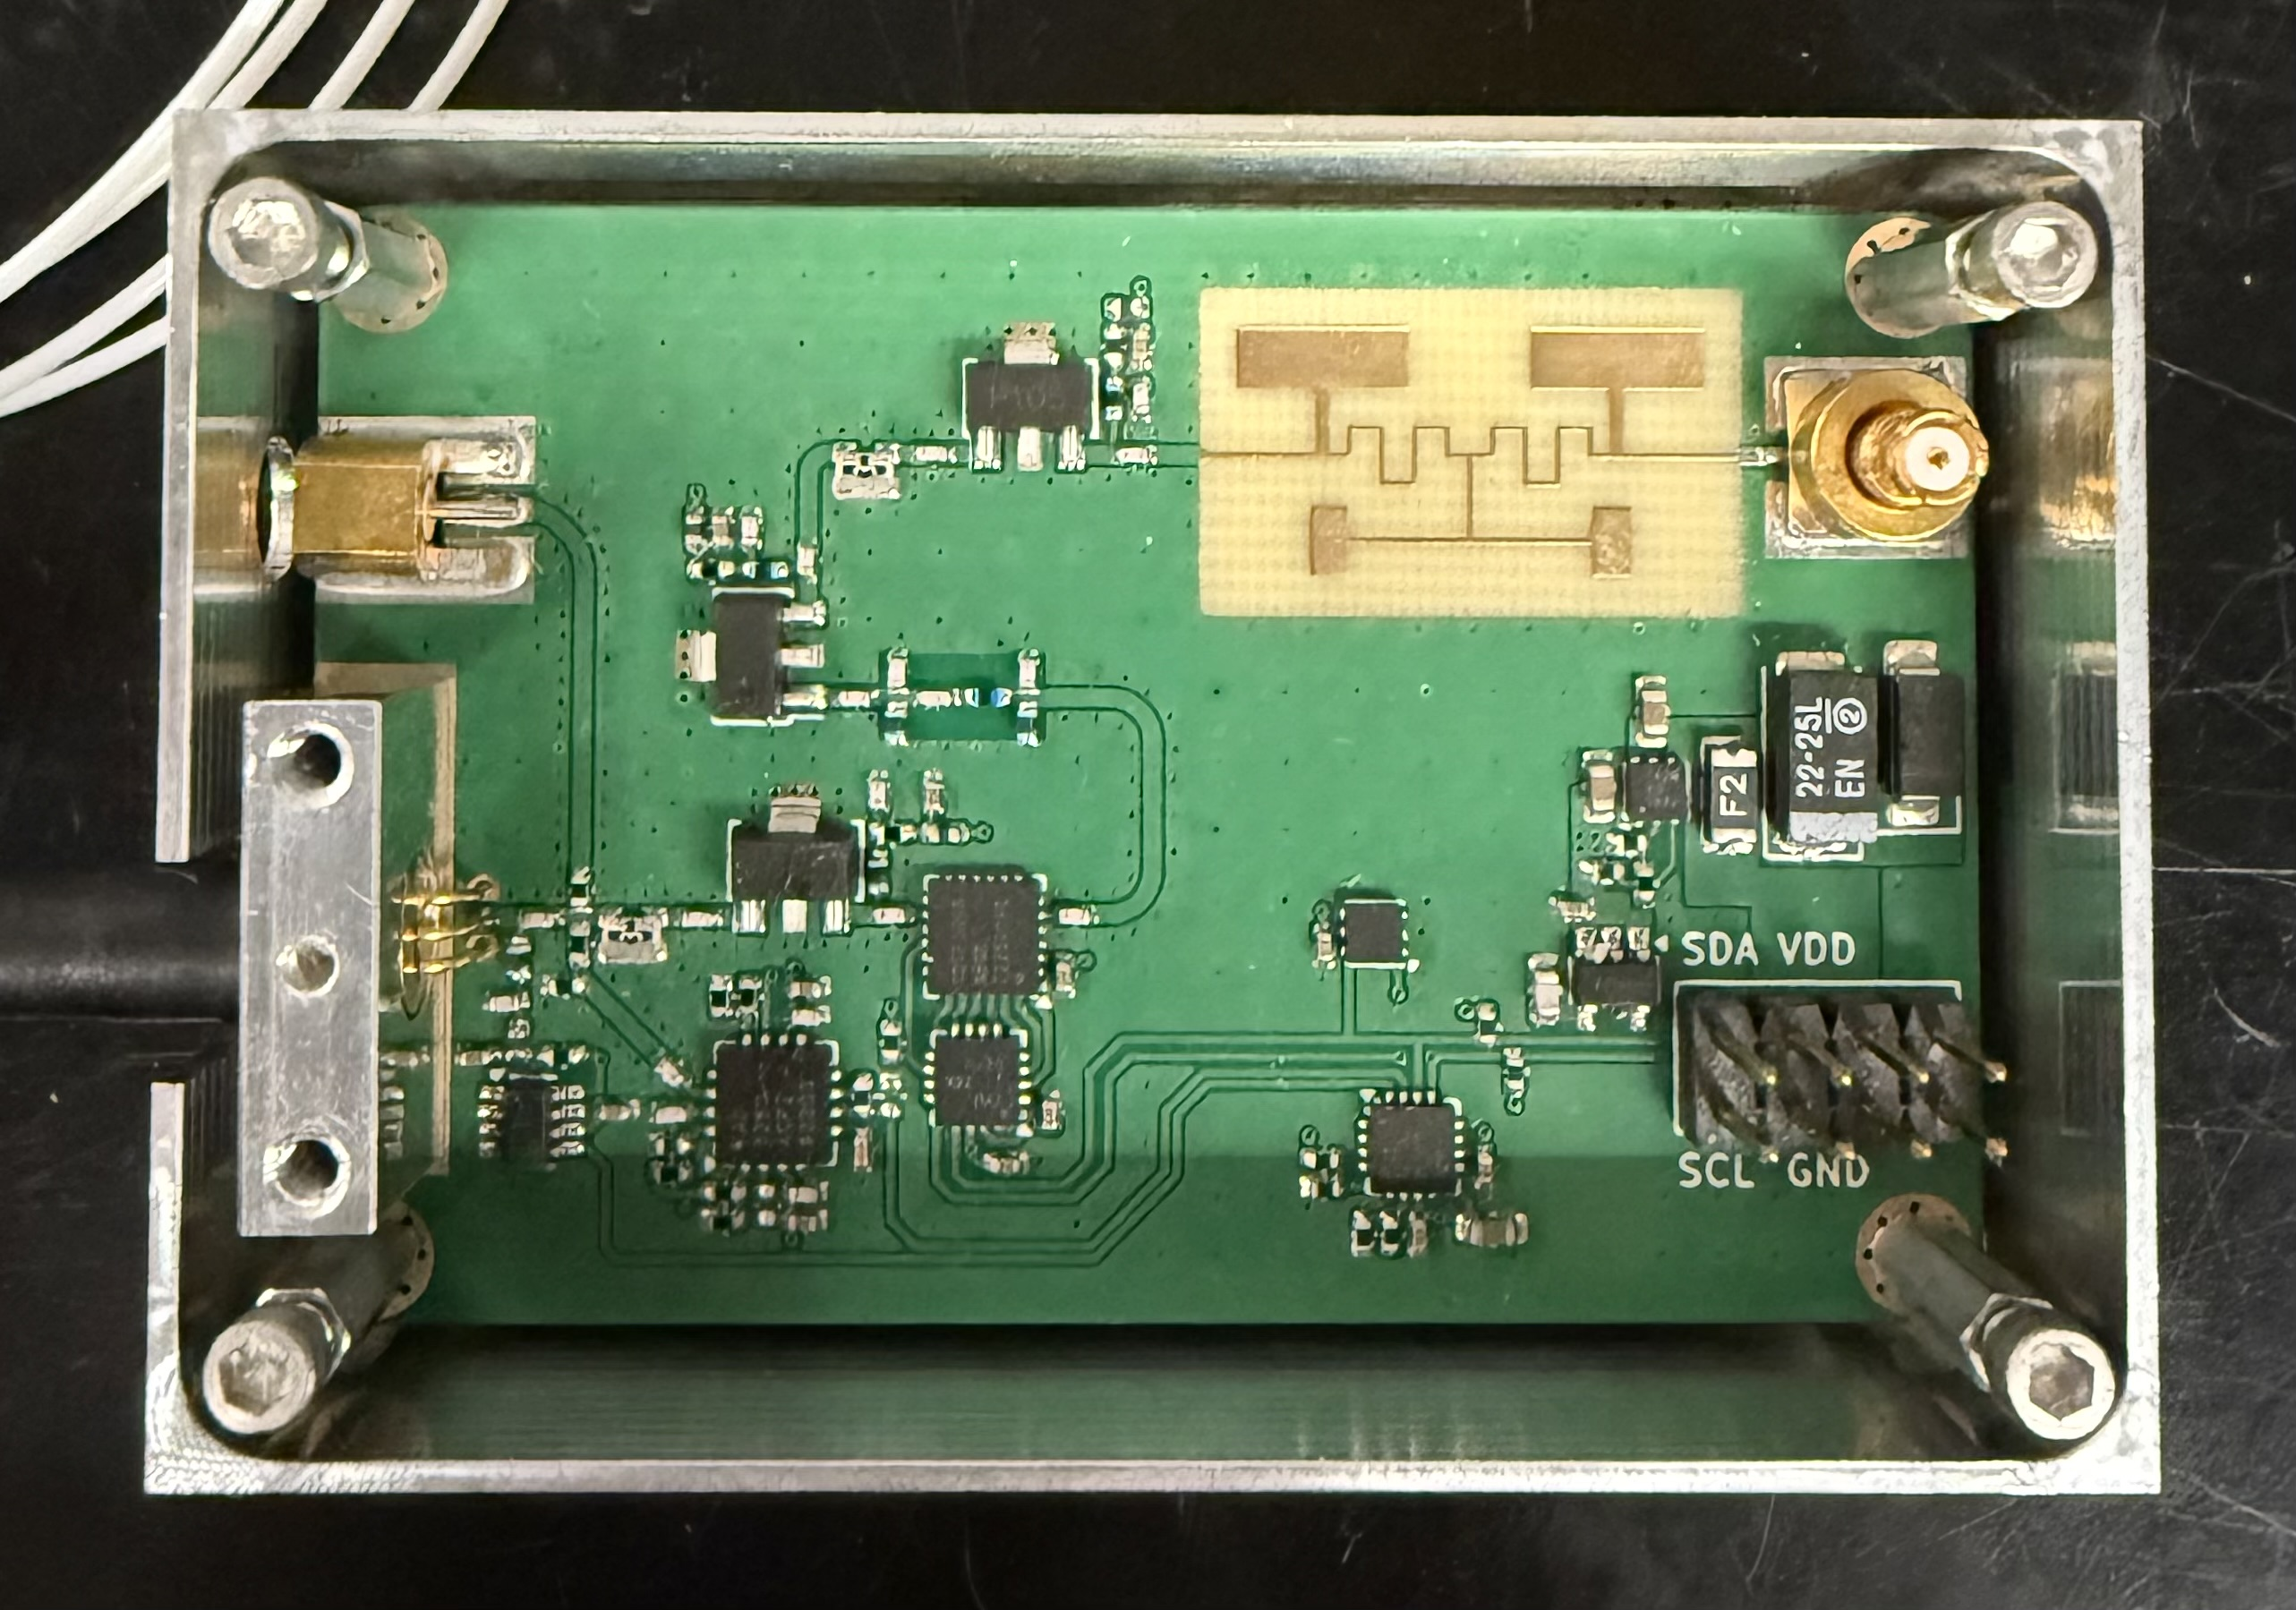
\includegraphics[height=4cm]{figures/frx.jpg}}%
    \caption{FTX and FRX PCBs}%
    \label{fig:ftx_frx}%
\end{figure}

To implement the analog signal path, we designed two printed circuit boards, shown in \autoref{fig:ftx_frx}.
These boards are the fiber transmitter (FTX) at the antenna station and the fiber receiver (FRX) at the central processing facility.
Both of these boards include monitor and control capabilities, measuring board currents, temperatures, and controlling digital step attenuators and bias currents.
This interface is achieved via an I$^2$C serial interface, whose digital lines are heavily filtered and will be disabled during observations.

\subsubsection{FTX}
The FTX board consists of three stages of amplification with a collection of filters and attenuators.
The laser bias is provided by a controlled current source, whose set point is controlled by a digital potentiometer.
The laser's anode is connected to the case, which implies we must drive the laser using a negative supply voltage.
Controlled current sources that allow for this are uncommon, motivating a custom design.
The design allows for a current selection between \qty{0}{\mA} and \qty{50}{\mA}, covering the full range of acceptable currents for the AGx laser.

In addition to the laser control, the FTX includes a connection point for an external filter.
In the current design stage, it is unclear if we will require much filtering besides shaping the 1280-1530 MHz bandpass.
In earlier stages of the project, strong interference causing significant distortion was a top concern.
The current RFI environment of the DSA-2000 site seems to indicate that no additional filtering will be required.
Nevertheless, the option to add the filters will remain if this situation changes.

The FTX board itself is housed inside an RFI-tight container, with feed-through connections for the RF, digital, and power signals.
The switching power supply for the board is housed on the outside of the enclosure to prevent switching noise from leaking into the signal path.
Each box contains electronics for both polarizations.

\subsubsection{FRX}

At the receiving side, the FRX module is a daughter board to the ``radio camera frontend'' or RCF.
The RCF is a larger card that hosts the ADCs and FPGA and fits into a 10-unit Eurocard subrack.
Two FRXes must then fit on a standard height card (\qty{100}{\mm}), with some gap for edge interfaces.
The RF signals out of the FRXes are connected to the digitizers on the RCF using a standard SMP board-to-board connector.
The FRXes are shielded with an aluminum cover that encloses the modules and are electrically connected to a ground plane on the RCF PCB.
The signals are routed on inner layers of the RCF PCB, so the FRX boards are surrounded by ground on all sides, except for a small slit that allows the fiber to exit.
The fiber pigtail is connected to the front panel of the card with a standard fiber interface.

The design of the FRX card was straightforward, with a standard assortment of filters and amplifiers.
Perhaps the most interesting component is the distributed low pass antialiasing filter at the output.
This filter is an inverse-Chebyshov low pass filter that has been optimized in physical area.
The center resonator was split in half and folded inwards to minimize space.

\section{LNA Improvements}

As the project progresses, the DSA-2000 team has been charged with pushing the performance even further, both in terms of what can be achieved before final design review and as avenues for future upgrades.
As the goal is to continue maximizing survey speed, we want to exhaust all options to reduce system noise within our budget.

For the current frequency range, there is very little we can do to improve the noise from a circuit design perspective.
The presented LNA from \autoref{ch:lna} is close to the theoretical minimum noise of the transistor, with typical losses of the matching network.
While this design is optimal for room temperature operation, it could benefit from cooling, as is the case for any transistor.
The entire premise of the ambient temperature LNA was to avoid cooling, but we can accomplish some cooling using Peltier microcoolers without resorting to expensive cryogenics.
Additionally, the noise of the amplifier is dependent on the source impedance presented by the feed.
As such, the design of the LNA input matching network could be modified to provide a better match to the feed instead of to \qty{50}{\ohm}.
The following section discusses these two potential improvements.

\subsection{Active Cooling}

Thermoelectric cooling of LNAs is a well-known approach~\cite{caoCoolingLowNoise2013} for improving an amplifier's noise.
However, most implementations of this strategy involve ``bulk'' cooling, where the entire amplifier assembly is cooled.
The power required for bulk cooling to achieve reasonable noise improvements can be significant.
Additionally, the hot-side of the cooler would need a large heat sink and fan for thermal management, adding size, weight, and power.
An alternative for hybrid amplifiers is to cool only the first-stage transistor, as that has the highest impact on the LNA's noise.
These transistors are very small and low power, requiring significantly less cooler power than what would be required to achieve the same noise improvement in bulk cooling.
Modern advancements in miniaturization of Peltier coolers for optoelectronics\footnote{Typically used for lasers in high-speed digital communication} have dramatically lowered cost and improved performance.
As such, we have designed an amplifier with an embedded microcooler for the first stage transistor to improve the noise without significant impact to cost or power consumption.
Variants on this idea have been shown before~\cite{schreuderLocalizedLNAVooling2006}, but have been limited to MMIC-based amplifiers, which require a larger cold-side area and cooling capacity.

The potential noise gains, however, need to be weighed against the complications that could arise due to creating a below-freezing point inside the amplifier.
This presents a formidable design challenge, as the goal for the project is to have an exceptionally low mean-time-to-failure.
If water vapor were to leak into the chassis, it would freeze over the transistor and result in failures.
To prevent this, we need to design an LNA that is hermetically sealed, which adds complexity and cost.
The improvement in survey speed, however, could be substantial depending on what is achievable and may outweigh the added engineering costs.

The current LNA design biases the transistor at a power of \qty{8}{\mW} (\qty{0.5}{\V} at \qty{16}{\mA} of drain current).
Models for this transistor at \qty{2}{\GHz} indicate a minimum noise temperature of \qty{7}{\K} at \qty{300}{\K} ambient and \qty{0.6}{\K} at \qty{15}{\K} ambient.
This results in a noise slope of about \qty{1}{\K} per \qty{45}{\K} change in ambient temperature.
To improve our amplifier by \qty{1}{\K}, we can integrate a small single-stage microcooler to generate the \qty{45}{\K} differential.

To fully estimate the heat load that we would need to cool, we must account for heat introduced from the short wire bonds.
We can compute this via
\begin{equation}
    Q_\text{Wires} = NK\frac{S}{L}\Delta T \,,
\end{equation}
where $N$ is the number of wires, $K$ is the wire material thermal conductivity, $S$ is the wire cross-sectional area, $L$ is the wire length, and $\Delta T$ is the temperature differential.
If we require $N=$ \num{5}, \qty{20}{\micro\m} diameter ($S$ \qty{=2.54e-10}{\m^2}) wire bonds (three for the transistor and two for the thermistor) made of gold ($K$ \qty{=314}{\W\per\m\per\K}) with an average length of $L$ \qty{=500}{\micro\m} across the $\Delta T$ of \qty{45}{\K}, we have an additional heat load of \qty{36}{\mW}.
This implies that the bulk of the required cooling capacity comes from the wire bonds and not the transistor.

As the $\Delta T$ produced by a Peltier cooler behaves non-linearly under different heat loads, a bit of trial and error is required to estimate their performance properly.
Estimations from the manufacturer\urlfootnote{https://www.tec-microsystems.com/} for their \texttt{1TC22-0044-25.H} model predicts a maximum $\Delta T$ of just beneath \qty{30}{\K} for \qty{45}{\mW} of heat.
With this $\Delta T$, however, the cooling requirement will be smaller as the heat from the wire bonds is less due to the lower temperature differential.
In this scenario, we can compute a total wire bond head load of \qty{32}{\mW}, which would induce a new $\Delta T$ closer to \qty{40}{\K}.
This all implies we can expect a measured $\Delta T$ of between \qty{30}{\K} and \qty{40}{\K}.

\begin{figure}[ht!]%
    \centering
    \subfloat{
        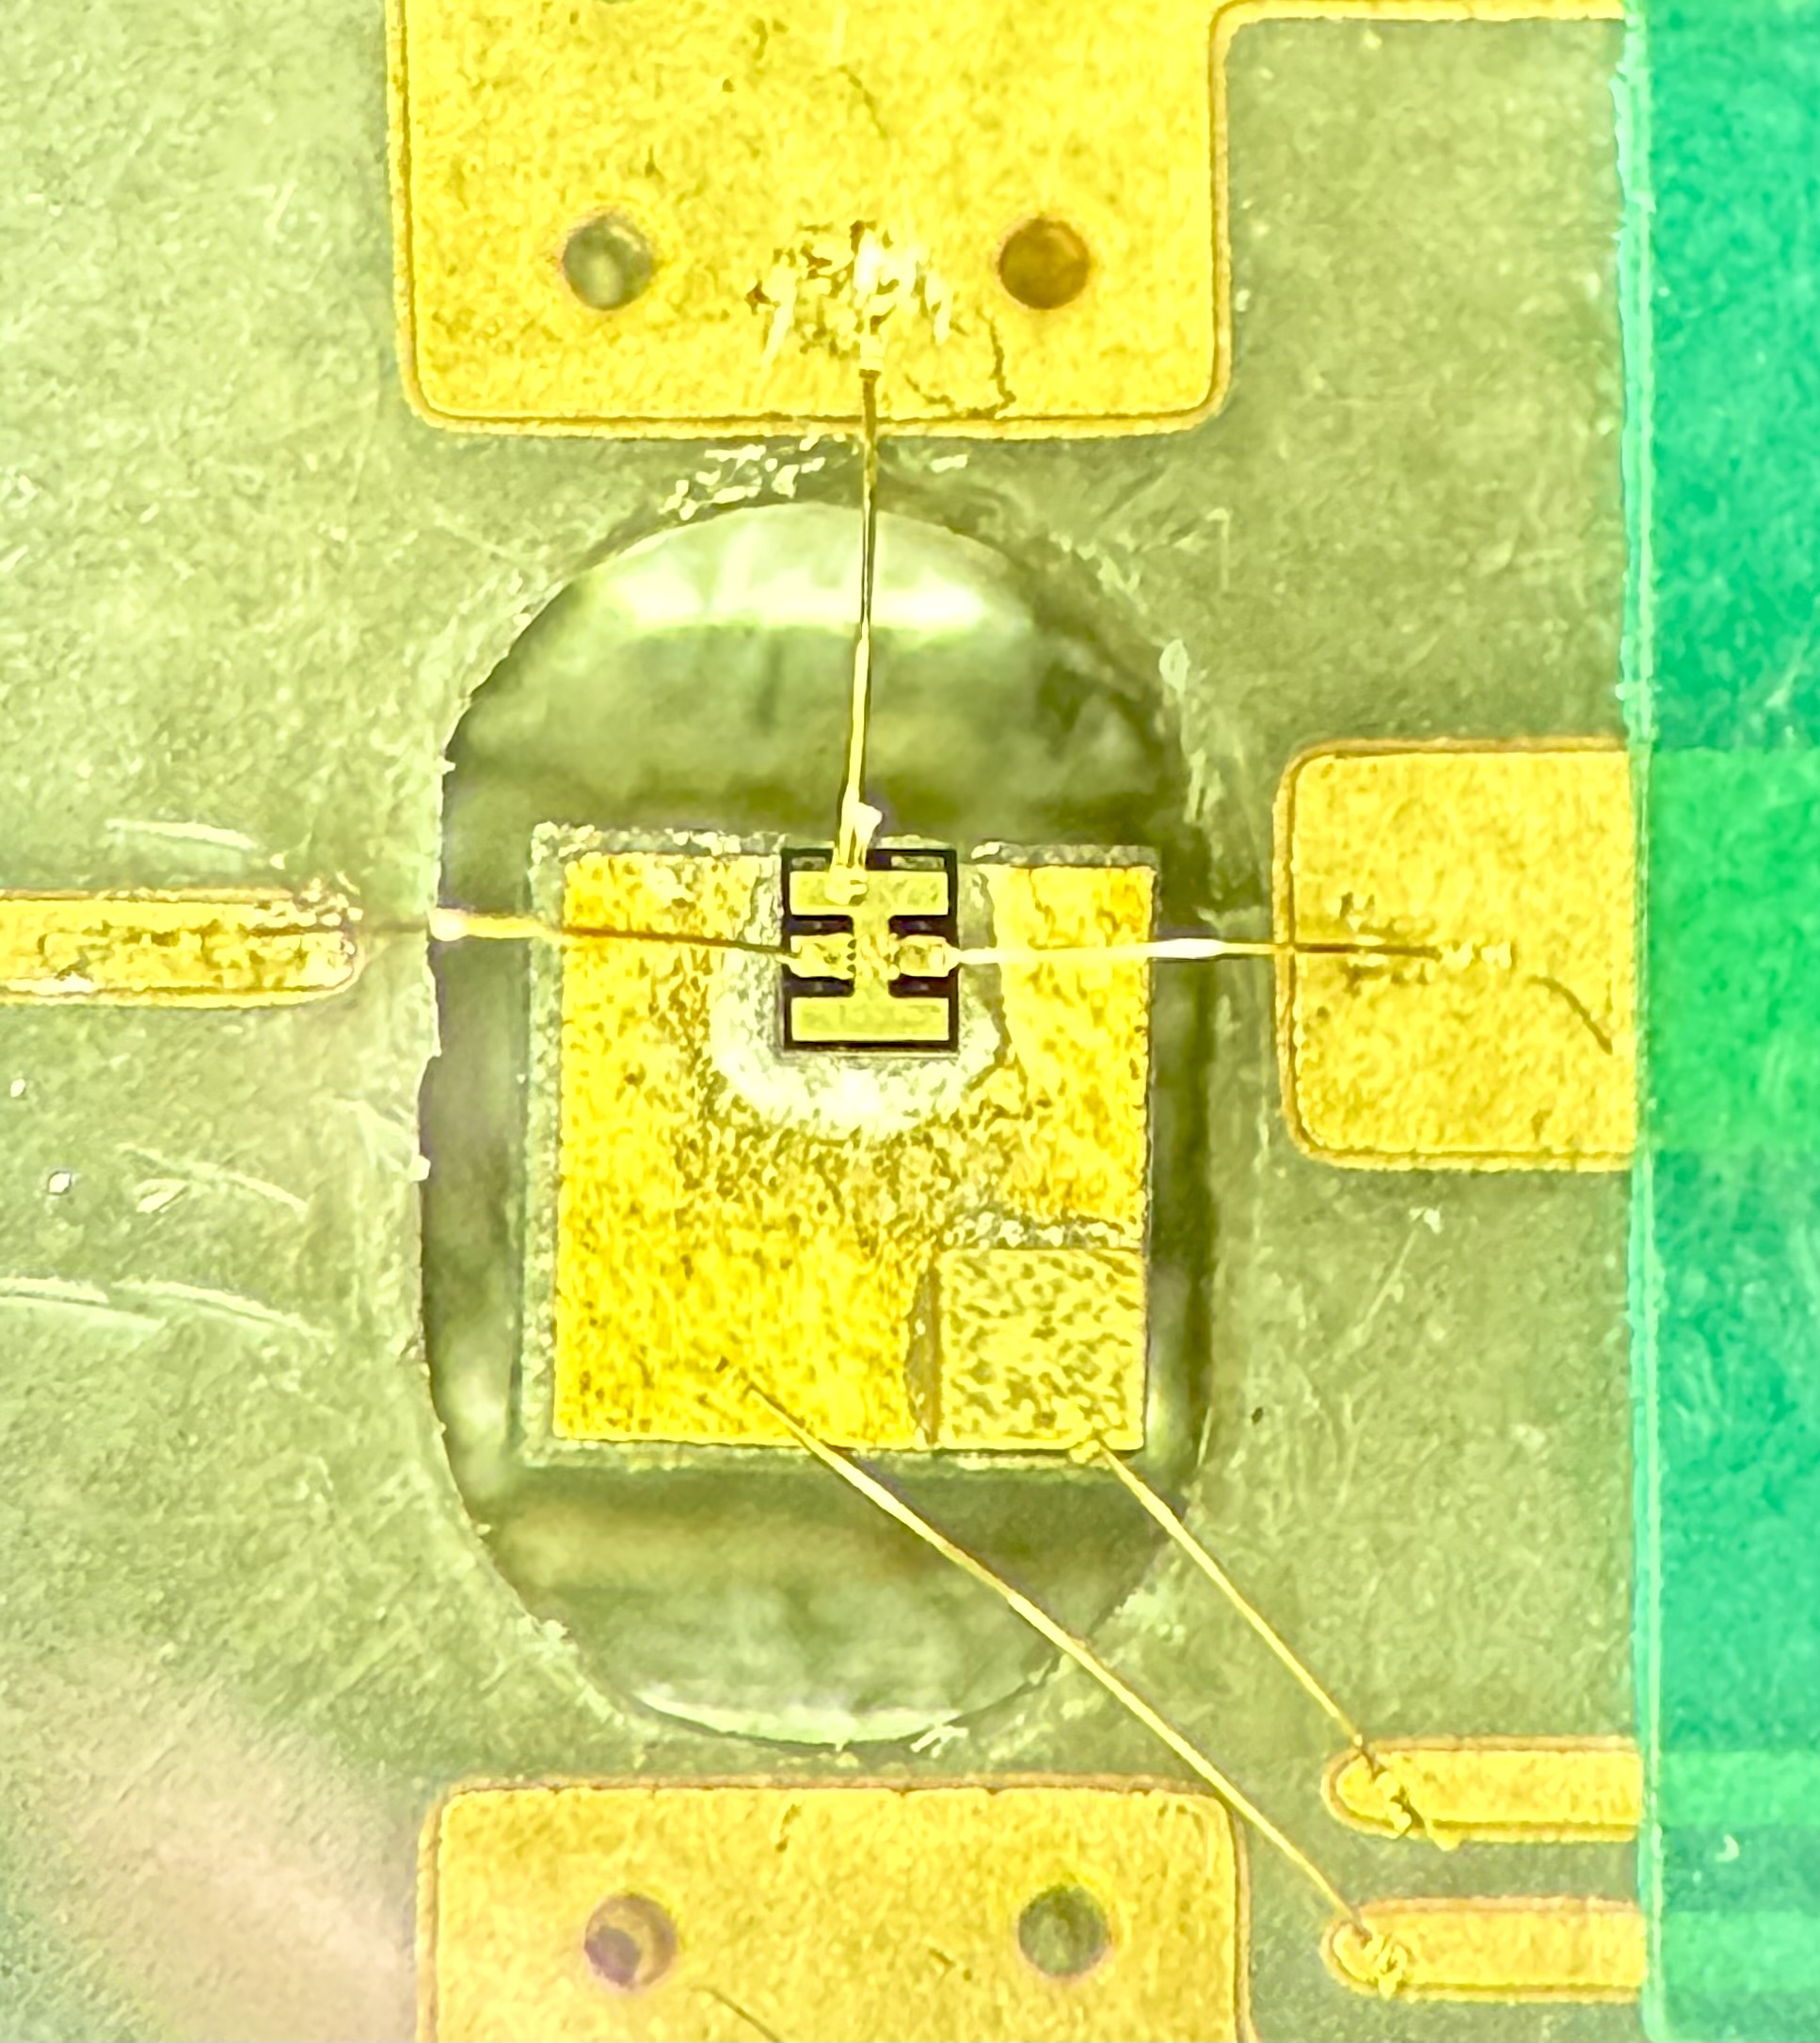
\includegraphics[height=6cm]{figures/tec.jpg}
    }
    \subfloat{
        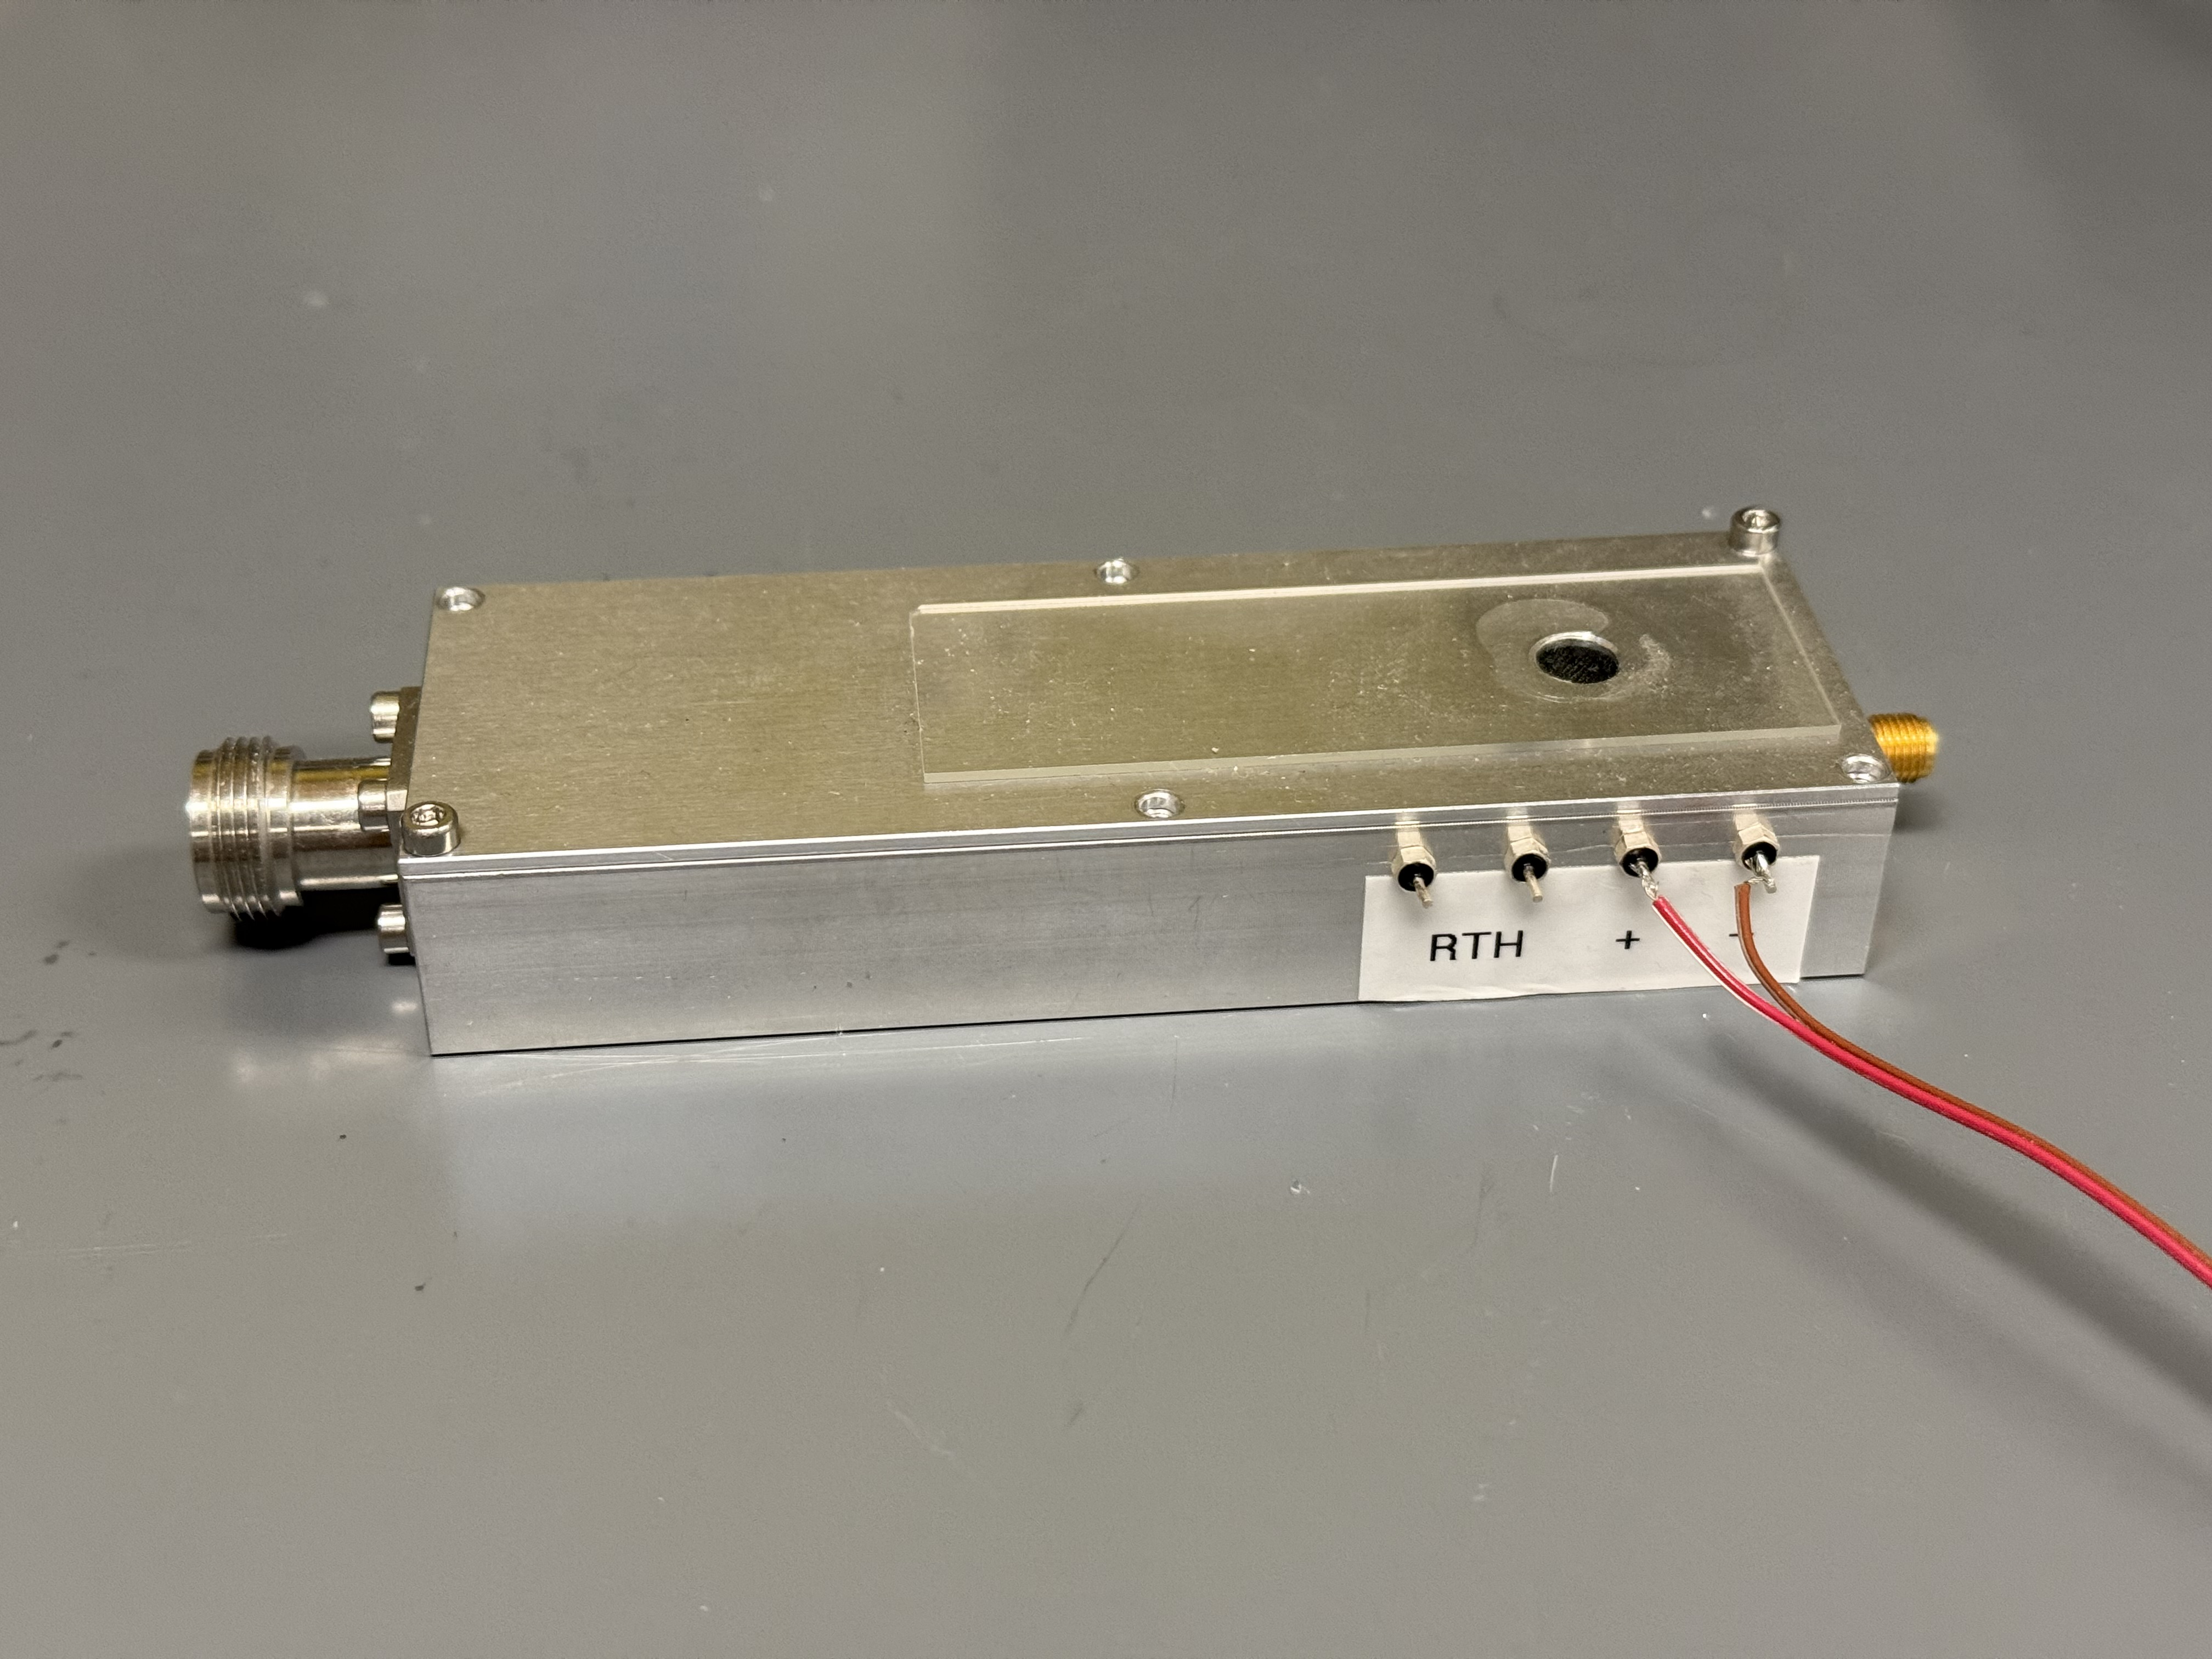
\includegraphics[height=6cm]{figures/cooled_amp.jpg}
    }%
    \caption{Bonded transistor on microcooler and constructed cooled amplifier}
    \label{fig:lna_cooling}%
\end{figure}

We constructed a copy of the amplifier described in \autoref{ch:lna}, but with an embedded microcooler.
While this amplifier was not hermetically sealed, two holes were added at either end, with dry nitrogen pumped through one side.
Additionally, a hole and microscope slide was added to the lid to observe the first stage transistor under cooling to watch for ice formation.
The microcooler was powered via an independent supply, and a thermistor was mounted to the cold-stage, adjacent to the transistor to monitor the temperature.
Finally, we performed the precision noise measurement described in \autoref{ch:lna}.
A close-up picture of the bonded transistor (center) and thermistor (bottom right) on the microcooler and assembled amplifier is shown in \autoref{fig:lna_cooling}.
The transistor's wire bonds from left to right are the gate, source, and drain.

With zero power applied to the microcooler, we measured a thermistor temperature of \qty{30}{\C}.
With the cooler powered to its maximum current, we measured a thermistor temperature of \qty{-10}{\C}, for a $\Delta T$ of \qty{40}{C}.
The LNA noise temperature dropped by an average of about \qty{0.75}{\K}, shown in \autoref{fig:cooled_noise}, which is very close to the predicted \qty{0.89}{\K} and well within the error for this measurement.

While the experiment was a success, eventually ice did start to form on the first stage transistor, destroying the fragile air bridges.
Work on this solid-state cooling approach needs further investigation in environmental control, especially as it pertains to mass-manufacture for the 4000 LNAs that would eventually need to be built.
Additionally, our original estimations of the heat load which influenced the sizing of the microcooler did not include the heat load of the wire bonds.
The manufacturer has suggested a new custom part, \texttt{1TC22-0040-21.H}, which should have a higher $\Delta T$ of about \qty{50}{\K} under our heat load of \qty{\approx40}{\mW}.
We could also investigate two-stage coolers for significantly more cooling capacity, but with a downside of doubling the cross-sectional area of the cold-stage.
This would increase wire bond length which would reduce the heat load, but add significant inductance which will alter our matching network.

\newpage

\begin{figure}[ht!]
    \centering
    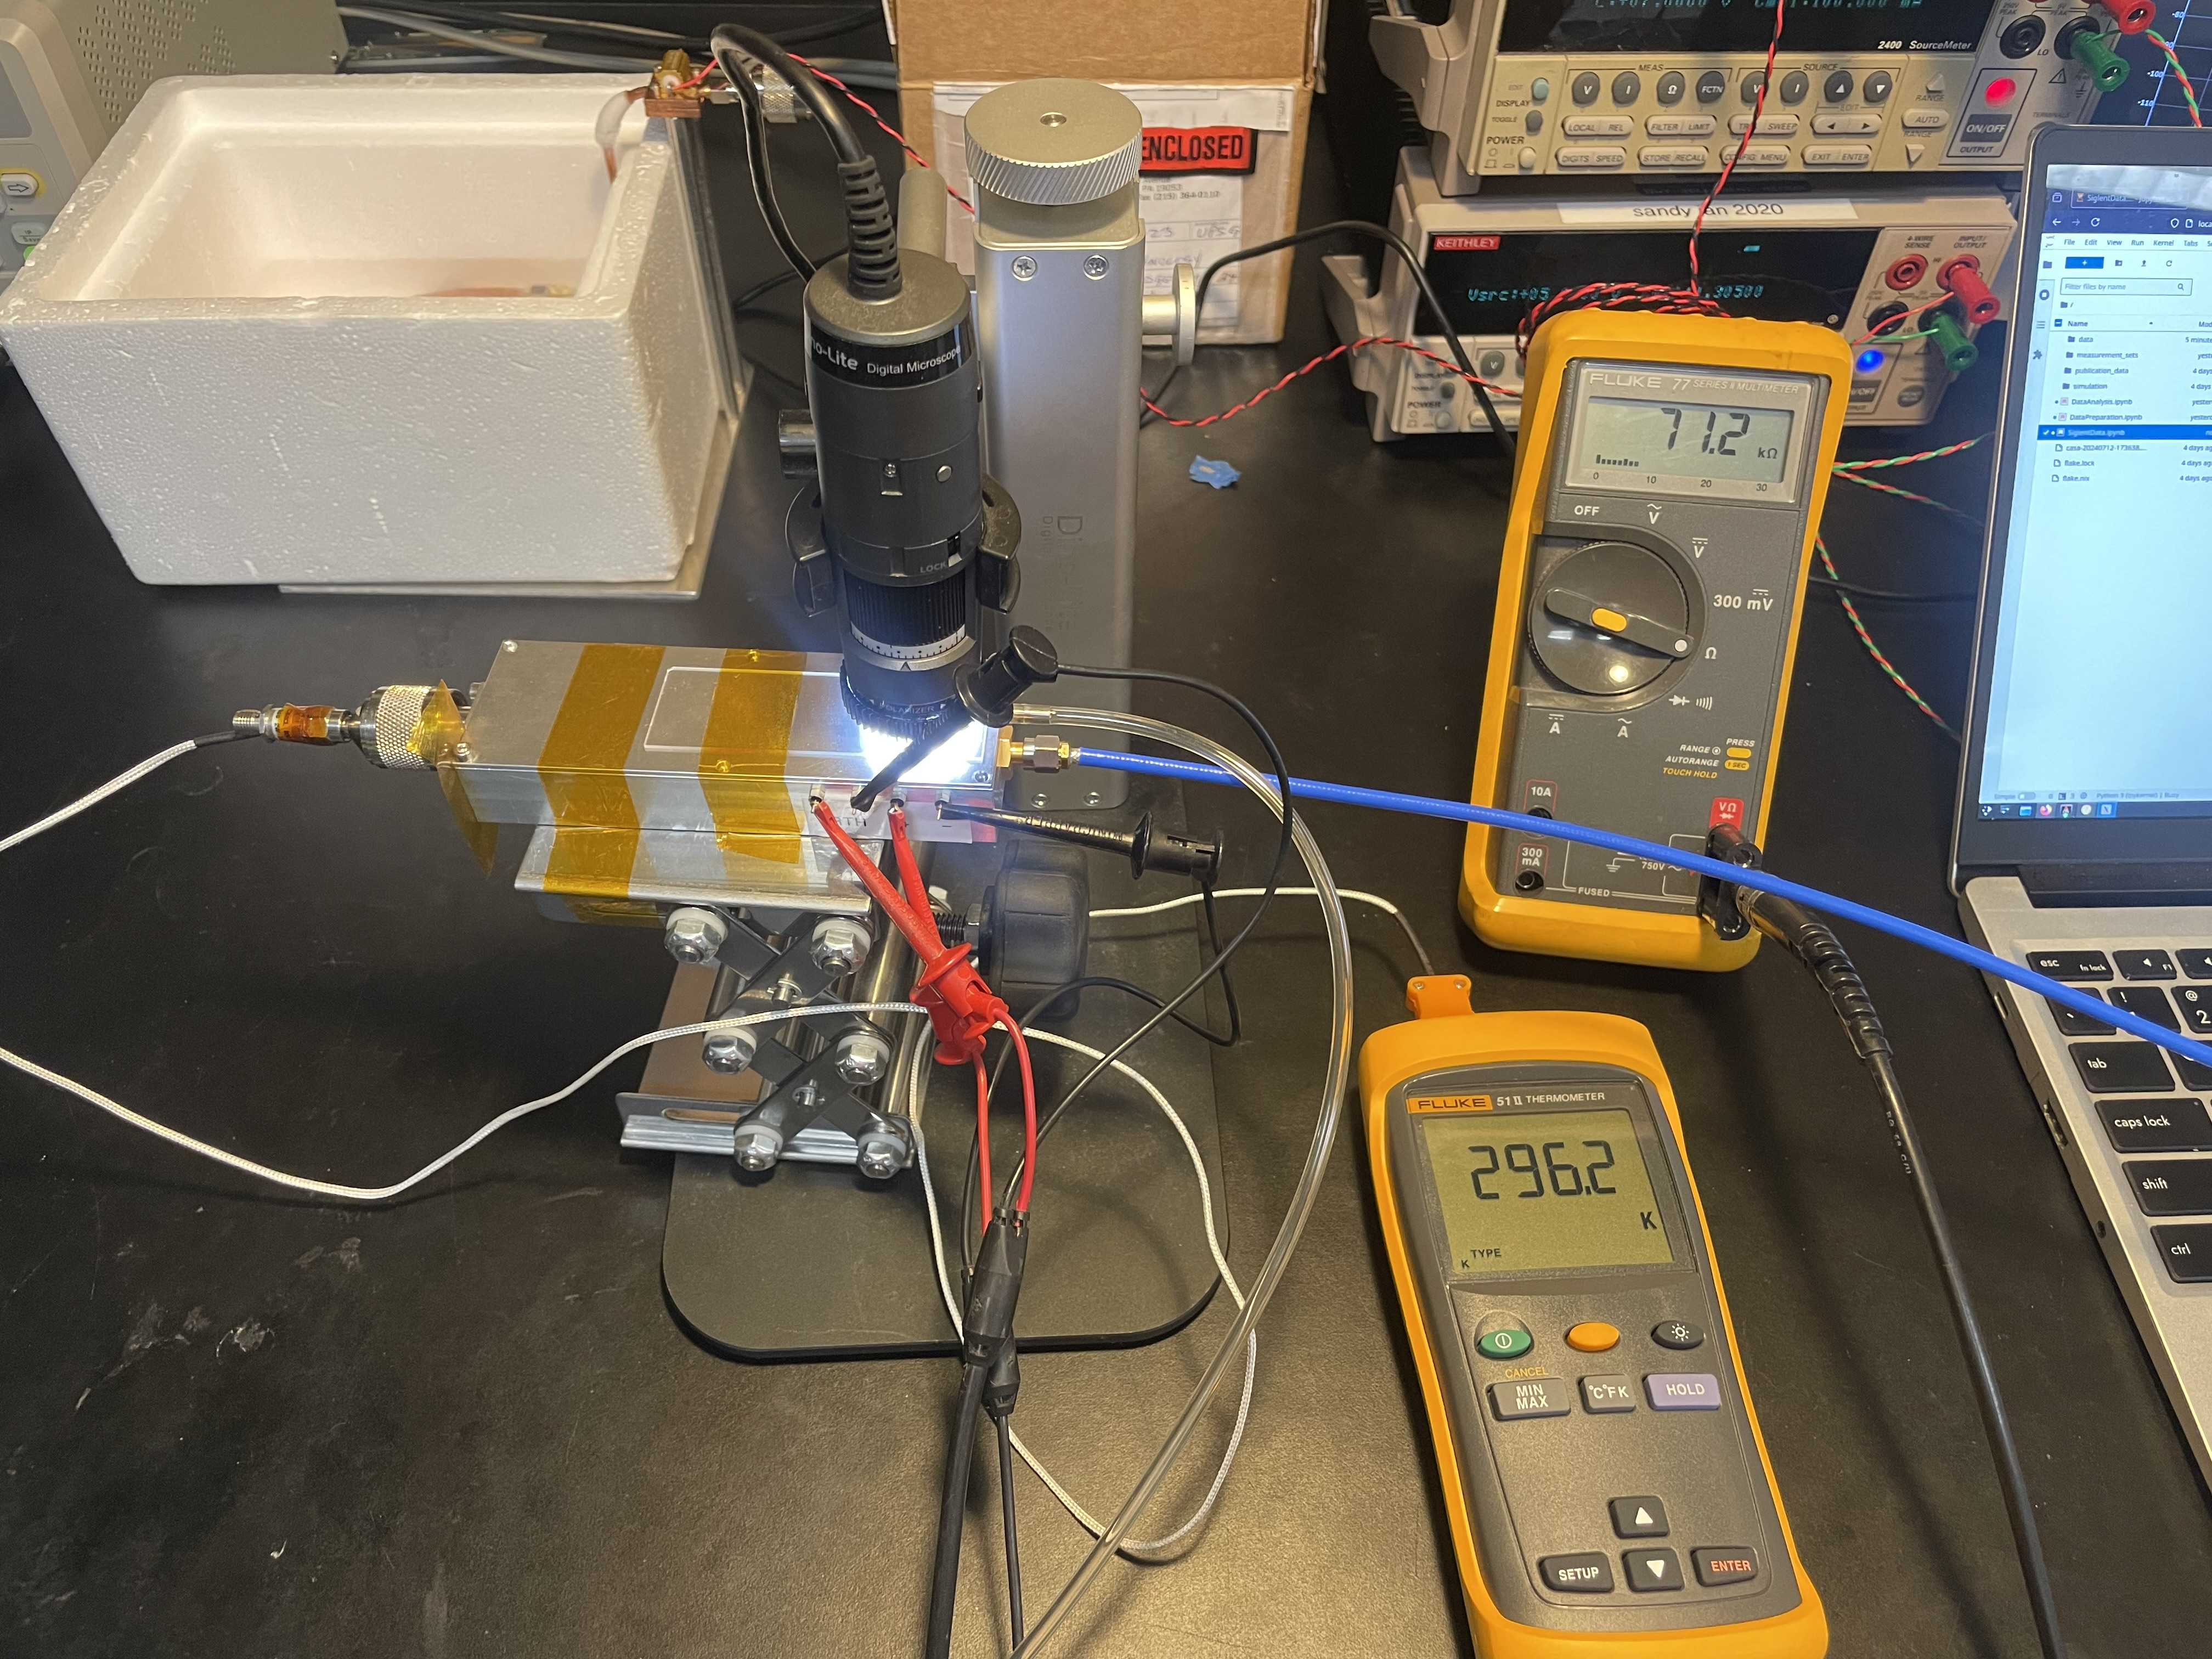
\includegraphics[width=0.8\linewidth]{figures/noise_test.jpg}
    \caption{Test setup for cooled amplifier noise measurements}
    \label{fig:noise_test}
\end{figure}

\begin{figure}[ht!]
    \centering
    \includestandalone[mode=buildnew]{figures/cooled_noise}
    \caption{Measured noise temperature of cooled amplifier}
    \label{fig:cooled_noise}
\end{figure}

\newpage

\subsection{Optimization of LNA Input Matching Network to Feed Impedance}

All our amplifier designs up to this point are intended to operate in a \qty{50}{\ohm} system, but the impedance presented by the feed is not \qty{50}{\ohm}.
The feed has return loss greater than \qty{10}{\dB} over much of the band, but the mismatch at the band edges significantly degrades the noise.

To reduce the effect of the feed impedance ``pulling'' the noise, we can design a matching network that is optimized for the feed impedance.
If the feed impedance were a large deviation from \qty{50}{\ohm}, it would be difficult to validate performance in the lab, as all the noise experiments are done in a \qty{50}{\ohm} system.
However, as the feed was intended to match to \qty{50}{\ohm}, we only have to compensate for a small difference in impedance, leaving the \qty{50}{\ohm} bench test more than satisfactory for validating performance.

Performing the co-optimization follows the work from \autoref{ch:lna}, with a small modification made to the definition of the noise goal in the cost expression.
Before, we were simply using $S_{22}$ of the nonuniform input matching network as the source reflection coefficient $\Gamma_S$ needed to compute the noise via \autoref{eq:noise_f}.
Now, we take measured $S_{11}$ data of the feed and compute $\Gamma_\text{Out}$ via
\begin{equation}
    \Gamma_\text{Out} = S_{22} + \frac{S_{21}S_{12}\Gamma_S}{1 - S_{11}\Gamma_S} \,,
\end{equation}
where $\Gamma_S$ is the measured feed $S_{11}$ (assuming everything is normalized to the same reference impedance).

The current feed design~\cite{flygareWidebandFeedReflector2023, flygareWidebandLowLossFeed2024}, is a quad-ridge flared horn, following previous work at Caltech~\cite{akgirayNewTechnologiesDriving2013}.
This feed includes a dielectric lens and ``cake pan'' choke rings to optimize the illumination of the DSA-2000 reflector.
As the ridges form a balanced transmission line, there is a shorted-pin balun that transitions from coax.
This transition is then brought to the edge of the feed structure to a standard microwave connector.
In the current design, the LNA is attached directly to this connector, resulting in the feed and LNA as two separate line-replaceable units (LRUs).

While the separation of components is useful from a maintenance perspective, the long coax pin that attaches the connector to the throat of the feed introduces additional loss.
An alternative design is to embed the LNA into the feed, using the ridge as the enclosure for the LNA PCB.
This sidesteps the need for the long coax pin and allows us to start the matching network very close to the slotline transition.
We can accomplish this while maintaining two distinct LRUs by designing an LNA chassis that slots into the ridge and connects to a blind-mate pin.
The new LNA chassis has a silver-epoxied \qty{50}{\ohm} glass feed-through connector to connect to the internal blind-mate pin.
A lid gasket and hermetic output connector seal the assembly and allow for solid-state cooling.

\begin{figure}[ht!]
    \centering
    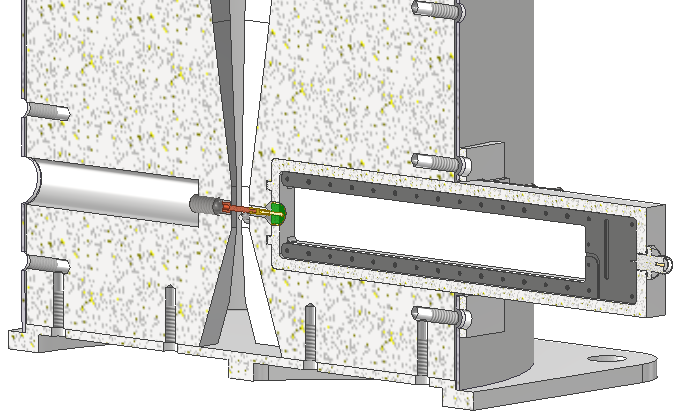
\includegraphics[width=\linewidth]{figures/feed_embed_cross_section.png}
    \caption{Cross-section of an LNA-embedded feed}
    \label{fig:feed_and_lna}
\end{figure}

\begin{figure}[ht!]
    \centering
    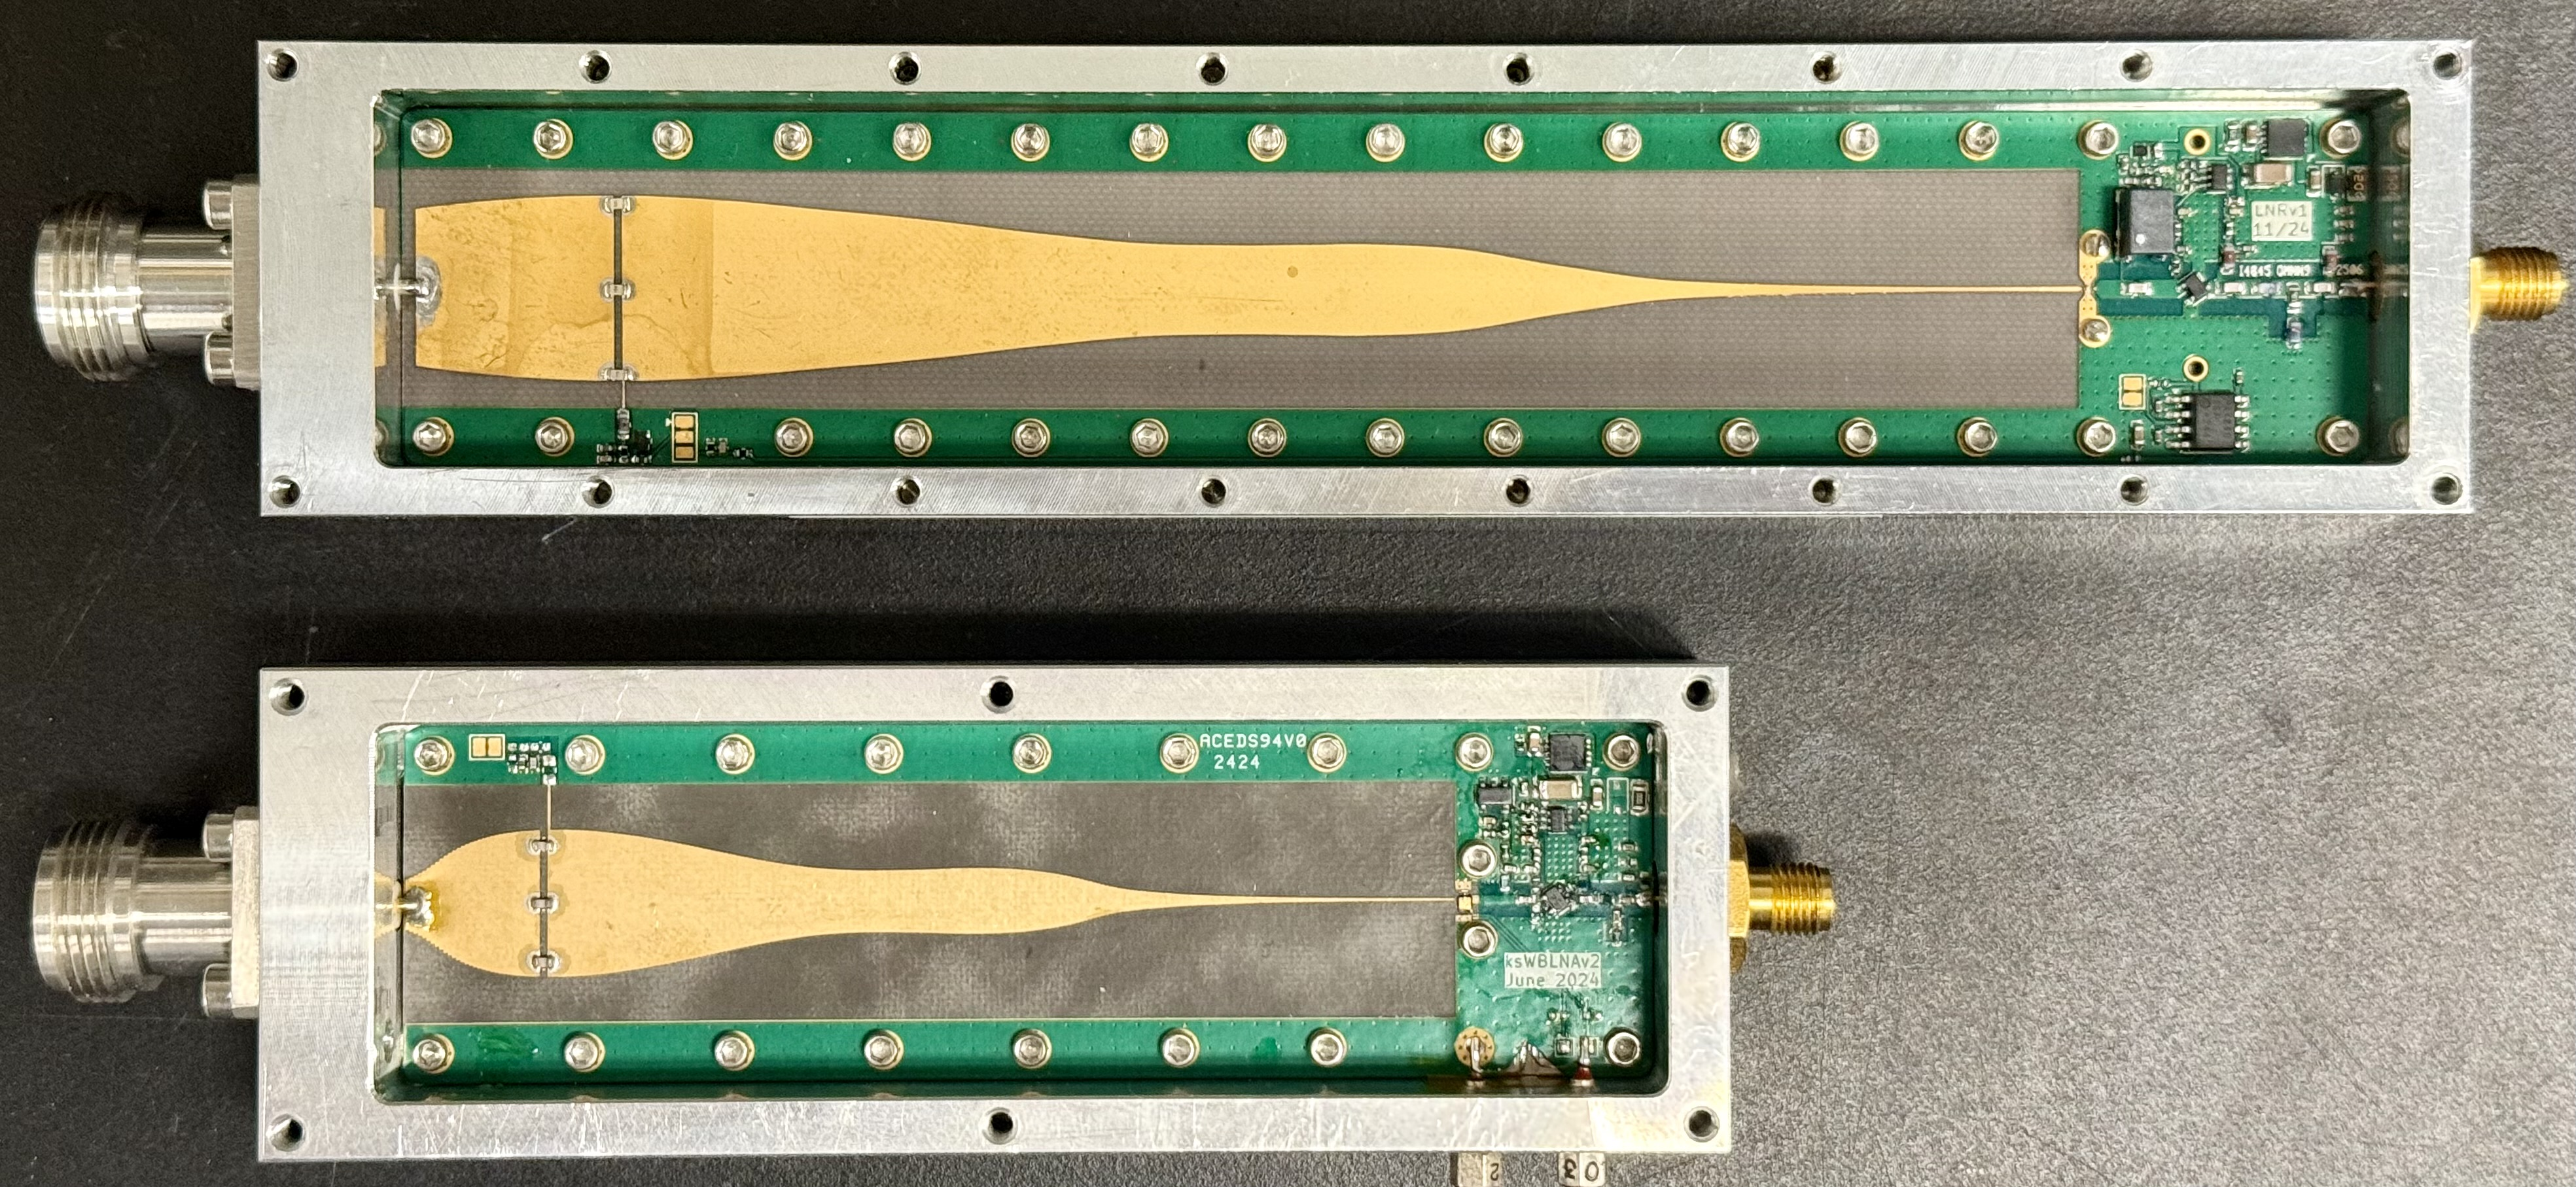
\includegraphics[width=\linewidth]{figures/lnr_v_lna.jpg}
    \caption{Comparison of the co-optimized LNA (in a test chassis) and the previous \qty{50}{\ohm} design}
    \label{fig:lnr_v_lna}
\end{figure}

The results from the optimization were surprising, as the optimal nonuniform line is significantly longer than the previous design.
This seems to indicate a shift in the optimum insertion loss versus noise match space.
At its core, the nonuniform matching approach requires long lines to successfully match complex loads~\cite{xiaoImpedanceMatchingComplex2002}.
As discussed in \autoref{ch:lna}, a well-matched, long line is at odds with the insertion loss of the line itself, implying that there exists some optimum compromise between the length of the line providing a quality noise match and the loss of the line.
When co-optimizing with the DSA-2000 feed, this optimum has shifted to favor longer lines.
In short, the design can tolerate the loss introduced from the longer line, as the noise otherwise introduced due to mismatch at the band edges is so great.

\begin{figure}[ht!]
    \centering
    \includestandalone[mode=buildnew]{figures/lnr_noise}
    \caption{Simulated noise temperature of co-optimized and original LNA designs given a simulated feed source impedance}
    \label{fig:lnr_sim_noise}
\end{figure}

The simulated equivalent noise temperatures for the previous design and the new design are presented in \autoref{fig:lnr_sim_noise}.
Although the difference in mean noise temperature is small (\qty{\approx1}{\K}), the improvement in noise from \qty{700}{\MHz} to \qty{800}{\MHz} is massive.
As survey speed is $\propto\lambda^2$, this improvement in the low frequency performance is huge.